\documentclass[11pt,a4paper,twocolumn]{report}
\usepackage{thesisstyle}
\renewcommand{\thesisauthors}{Felix Laga}
\renewcommand{\bibname}{References}
\graphicspath{{figures/}}
% Generated by paper/make_numbers.py from research/spinodal_onset/outputs.
\newcommand{\BAMOneFigure}{1.5}
\newcommand{\BAMOneInflated}{2.4}
\newcommand{\BAMOneNoVolume}{1.5}
\newcommand{\BAMOnePhaseComp}{6.1}
\newcommand{\BAMOnePhaseHom}{1.4}
\newcommand{\BAMOneTable}{1.5}
\newcommand{\ChiCompMFour}{15.1}
\newcommand{\ChiCompMOneFigure}{18.5}
\newcommand{\ChiCompMOneInflated}{17.8}
\newcommand{\ChiCompMOneNoVolume}{13.8}
\newcommand{\ChiCompMOnePhaseComp}{11.7}
\newcommand{\ChiCompMOnePhaseHom}{0.0}
\newcommand{\ChiCompMOneTable}{12.2}
\newcommand{\ChiCompMThree}{13.4}
\newcommand{\ChiCompMTwo}{5.0}
\newcommand{\ChiHomMFour}{13.4}
\newcommand{\ChiHomMOneFigure}{21.8}
\newcommand{\ChiHomMOneInflated}{19.1}
\newcommand{\ChiHomMOneNoVolume}{2.3}
\newcommand{\ChiHomMOnePhaseComp}{0.0}
\newcommand{\ChiHomMOnePhaseHom}{10.0}
\newcommand{\ChiHomMOneTable}{21.9}
\newcommand{\ChiHomMThree}{15.1}
\newcommand{\ChiHomMTwo}{18.8}
\newcommand{\ChiMFour}{48}
\newcommand{\ChiMOneFigure}{58}
\newcommand{\ChiMOneInflated}{40}
\newcommand{\ChiMOneNoVolume}{26}
\newcommand{\ChiMOnePhaseComp}{21}
\newcommand{\ChiMOnePhaseHom}{10}
\newcommand{\ChiMOneTable}{54}
\newcommand{\ChiMThree}{49}
\newcommand{\ChiMTwo}{45}
\newcommand{\ChiPhaseMFour}{20.0}
\newcommand{\ChiPhaseMOneFigure}{17.9}
\newcommand{\ChiPhaseMOneInflated}{3.3}
\newcommand{\ChiPhaseMOneNoVolume}{10.4}
\newcommand{\ChiPhaseMOnePhaseComp}{9.0}
\newcommand{\ChiPhaseMOnePhaseHom}{0.1}
\newcommand{\ChiPhaseMOneTable}{20.2}
\newcommand{\ChiPhaseMThree}{20.1}
\newcommand{\ChiPhaseMTwo}{21.5}
\newcommand{\FhMFour}{47}
\newcommand{\FhMOneFigure}{49}
\newcommand{\FhMOneInflated}{58}
\newcommand{\FhMOneNoVolume}{49}
\newcommand{\FhMOnePhaseComp}{65}
\newcommand{\FhMOnePhaseHom}{44}
\newcommand{\FhMOneTable}{48}
\newcommand{\FhMThree}{41}
\newcommand{\FhMTwo}{41}
\newcommand{\IntMFour}{144}
\newcommand{\IntMFourHi}{248}
\newcommand{\IntMFourHiNinetyFive}{479}
\newcommand{\IntMFourLo}{92}
\newcommand{\IntMFourLoNinetyFive}{59}
\newcommand{\IntMOneFigure}{92}
\newcommand{\IntMOneFigureHi}{122}
\newcommand{\IntMOneFigureLo}{69}
\newcommand{\IntMOneInflated}{220}
\newcommand{\IntMOneInflatedHi}{295}
\newcommand{\IntMOneInflatedLo}{157}
\newcommand{\IntMOneNoVolume}{86}
\newcommand{\IntMOneNoVolumeHi}{111}
\newcommand{\IntMOneNoVolumeLo}{64}
\newcommand{\IntMOnePhaseComp}{132}
\newcommand{\IntMOnePhaseCompHi}{198}
\newcommand{\IntMOnePhaseCompLo}{83}
\newcommand{\IntMOnePhaseHom}{65}
\newcommand{\IntMOnePhaseHomHi}{120}
\newcommand{\IntMOnePhaseHomLo}{23}
\newcommand{\IntMOneTable}{90}
\newcommand{\IntMOneTableHi}{115}
\newcommand{\IntMOneTableLo}{68}
\newcommand{\IntMThree}{87}
\newcommand{\IntMThreeHi}{111}
\newcommand{\IntMThreeLo}{67}
\newcommand{\IntMTwo}{42}
\newcommand{\IntMTwoHi}{68}
\newcommand{\IntMTwoLo}{24}
\newcommand{\IntRangeHi}{220}
\newcommand{\IntRangeLo}{42}
\newcommand{\MissMFour}{248}
\newcommand{\MissMOneFigure}{234}
\newcommand{\MissMOneInflated}{100}
\newcommand{\MissMOneNoVolume}{179}
\newcommand{\MissMOnePhaseComp}{167}
\newcommand{\MissMOnePhaseHom}{14}
\newcommand{\MissMOneTable}{249}
\newcommand{\MissMThree}{249}
\newcommand{\MissMTwo}{257}
\newcommand{\RhatMFour}{1.00}
\newcommand{\RhatMOneFigure}{1.01}
\newcommand{\RhatMOneInflated}{1.00}
\newcommand{\RhatMOneNoVolume}{1.00}
\newcommand{\RhatMOnePhaseComp}{1.05}
\newcommand{\RhatMOnePhaseHom}{1.00}
\newcommand{\RhatMOneTable}{1.00}
\newcommand{\RhatMThree}{1.00}
\newcommand{\RhatMTwo}{1.00}
\newcommand{\SlopeMOneFigure}{74}
\newcommand{\SlopeMOneInflated}{65}
\newcommand{\SlopeMOneNoVolume}{94}
\newcommand{\SlopeMOnePhaseComp}{100}
\newcommand{\SlopeMOnePhaseHom}{54}
\newcommand{\SlopeMOneTable}{74}
\newcommand{\TcMFour}{3265}
\newcommand{\TcMFourHi}{3319}
\newcommand{\TcMFourLo}{3230}
\newcommand{\TcMOneFigure}{3255}
\newcommand{\TcMOneFigureHi}{3281}
\newcommand{\TcMOneFigureLo}{3228}
\newcommand{\TcMOneInflated}{3412}
\newcommand{\TcMOneInflatedHi}{3477}
\newcommand{\TcMOneInflatedLo}{3347}
\newcommand{\TcMOneNoVolume}{3298}
\newcommand{\TcMOneNoVolumeHi}{3318}
\newcommand{\TcMOneNoVolumeLo}{3276}
\newcommand{\TcMOnePhaseComp}{3311}
\newcommand{\TcMOnePhaseCompHi}{3328}
\newcommand{\TcMOnePhaseCompLo}{3289}
\newcommand{\TcMOnePhaseHom}{3480}
\newcommand{\TcMOnePhaseHomHi}{3553}
\newcommand{\TcMOnePhaseHomLo}{3425}
\newcommand{\TcMOneTable}{3235}
\newcommand{\TcMOneTableHi}{3259}
\newcommand{\TcMOneTableLo}{3212}
\newcommand{\TcMThree}{3244}
\newcommand{\TcMThreeHi}{3277}
\newcommand{\TcMThreeLo}{3217}
\newcommand{\TcMTwo}{3221}
\newcommand{\TcMTwoHi}{3248}
\newcommand{\TcMTwoLo}{3196}
\newcommand{\UndefMFour}{0}
\newcommand{\UndefMOneFigure}{0}
\newcommand{\UndefMOneInflated}{0}
\newcommand{\UndefMOneNoVolume}{0}
\newcommand{\UndefMOnePhaseComp}{0}
\newcommand{\UndefMOnePhaseHom}{0}
\newcommand{\UndefMOneTable}{0}
\newcommand{\UndefMThree}{0}
\newcommand{\UndefMTwo}{0}
\newcommand{\XcMFour}{0.60}
\newcommand{\XcMOneFigure}{0.63}
\newcommand{\XcMOneInflated}{0.68}
\newcommand{\XcMOneNoVolume}{0.63}
\newcommand{\XcMOnePhaseComp}{0.72}
\newcommand{\XcMOnePhaseHom}{0.60}
\newcommand{\XcMOneTable}{0.63}
\newcommand{\XcMThree}{0.58}
\newcommand{\XcMTwo}{0.57}
\newcommand{\bumpFive}{-13.5}
\newcommand{\bumpFiveAbs}{13.5}
\newcommand{\bumpThree}{35.9}
\newcommand{\bumpThreeAbs}{35.9}
\newcommand{\bumpTwo}{250.4}
\newcommand{\bumpTwoAbs}{250.4}
\newcommand{\curvFracMeta}{46}
\newcommand{\curvFracOnePhase}{48}
\newcommand{\curvFracStable}{95}
\newcommand{\curvSdPooled}{25}
\newcommand{\curvT}{3200}
\newcommand{\designBestX}{0.35}
\newcommand{\designSdAfter}{75}
\newcommand{\designSdNow}{83}
\newcommand{\diffHiFiveOneFour}{$+$0.030}
\newcommand{\diffHiOneSixFive}{$+$0.053}
\newcommand{\diffLoFiveOneFour}{$-$0.073}
\newcommand{\diffLoOneSixFive}{$-$0.039}
\newcommand{\digMarker}{0.0006}
\newcommand{\digMax}{15}
\newcommand{\digRms}{2.3}
\newcommand{\draftdate}{29 October 2026}
\newcommand{\energyLowering}{2.98}
\newcommand{\eqFhThreeThousand}{61.4}
\newcommand{\fhPressureSpread}{$2\times10^{-10}$}
\newcommand{\fhPressureSpreadAll}{$7\times10^{-6}$}
\newcommand{\figHiFiveOneFour}{0.736}
\newcommand{\figHiOneSixFive}{0.629}
\newcommand{\figLoFiveOneFour}{0.514}
\newcommand{\figLoOneSixFive}{0.419}
\newcommand{\gramsWithheld}{18.4}
\newcommand{\indepMaxDiff}{$10^{-6}$}
\newcommand{\indepMaxDiffCrit}{0.11}
\newcommand{\indepRows}{6,888}
\newcommand{\maxRhat}{1.05}
\newcommand{\missHi}{257}
\newcommand{\missLo}{100}
\newcommand{\nCoolingRows}{10,827}
\newcommand{\nNativeSolves}{27}
\newcommand{\nOnsetRows}{20,664}
\newcommand{\nStressRows}{375}
\newcommand{\nTests}{288}
\newcommand{\oldFhFive}{39.0}
\newcommand{\oldFhTen}{39.0}
\newcommand{\oldFhTwo}{39.0}
\newcommand{\oldIntFive}{48}
\newcommand{\oldIntTen}{40}
\newcommand{\oldIntTwo}{53}
\newcommand{\oldTbFive}{3601}
\newcommand{\oldTbTen}{3001}
\newcommand{\oldTbTwo}{3962}
\newcommand{\oldThreshold}{1.01}
\newcommand{\oldTspFive}{3553}
\newcommand{\oldTspTen}{2961}
\newcommand{\oldTspTwo}{3908}
\newcommand{\pubChiComp}{71.3}
\newcommand{\pubChiHom}{111.4}
\newcommand{\pubChiPhase}{0.4}
\newcommand{\pubChiTotal}{183}
\newcommand{\pubFhFive}{65.5}
\newcommand{\pubFhTen}{65.5}
\newcommand{\pubFhTwo}{65.5}
\newcommand{\pubIntFive}{376}
\newcommand{\pubIntTen}{313}
\newcommand{\pubIntTwo}{414}
\newcommand{\pubMissOneSixFive}{35}
\newcommand{\pubTbBulkOneSixFive}{3465}
\newcommand{\pubTbFive}{3051}
\newcommand{\pubTbTen}{2542}
\newcommand{\pubTbTwo}{3356}
\newcommand{\pubTcFive}{3172}
\newcommand{\pubTcFiveOneFour}{3157}
\newcommand{\pubTcOneSixFive}{3526}
\newcommand{\pubTcTen}{2643}
\newcommand{\pubTcTwo}{3489}
\newcommand{\pubTcZero}{3700}
\newcommand{\pubThreshold}{1.40}
\newcommand{\pubTspFive}{2675}
\newcommand{\pubTspTen}{2229}
\newcommand{\pubTspTwo}{2942}
\newcommand{\pubWc}{9.36}
\newcommand{\pubXc}{0.720}
\newcommand{\slopeMinimum}{143}
\newcommand{\slopePublished}{106}
\newcommand{\stressFhHi}{66.3}
\newcommand{\stressFhLo}{64.4}
\newcommand{\stressIntHi}{504}
\newcommand{\stressIntLo}{329}
\newcommand{\tcAboveRunNearCritHigh}{157}
\newcommand{\tcAboveRunNearCritLow}{26}
\newcommand{\vModMid}{-1.94}
\newcommand{\vObsMid}{-1.00}
\newcommand{\vSigMid}{0.17}
\newcommand{\wrongFhFive}{36.1}
\newcommand{\wrongFhTen}{36.1}
\newcommand{\wrongFhTwo}{36.1}
\newcommand{\wrongIntFive}{42}
\newcommand{\wrongIntTen}{35}
\newcommand{\wrongIntTwo}{46}
\newcommand{\wrongTbFive}{3152}
\newcommand{\wrongTbTen}{2627}
\newcommand{\wrongTbTwo}{3468}
\newcommand{\wrongTspFive}{3111}
\newcommand{\wrongTspTen}{2592}
\newcommand{\wrongTspTwo}{3422}
\newcommand{\xMid}{0.588}


\hypersetup{pdftitle={Delayed Hydrogen Exsolution in Sub-Neptune Exoplanets under Magma-Envelope Coupling},
  pdfauthor={Felix Laga}}

\begin{document}

% ======================================================================= title page
\onecolumn
\begin{titlepage}
\newgeometry{onecolumn,left=2.0cm,right=2.0cm,top=1.0cm,bottom=1.2cm}
\sffamily
\vspace*{0pt}
\noindent\hspace*{-1.0cm}
\includegraphics[width=5.55cm]{kuleuven_logo.png}\par
\vspace{6.85cm}
{\raggedright\Huge Delayed Hydrogen Exsolution in\\[2pt]
Sub-Neptune Exoplanets under\\[2pt] Magma-Envelope Coupling\par}
\vspace{2.0cm}
{\Large Felix Laga\par}
\vspace{3.0cm}
\begin{flushright}\large
Research draft, building on the bachelor thesis\\
of F.~Laga \& S.~Vanhulle (2025)\\[8pt]
\textbf{Bachelor thesis supervisor:}\\
Dr.~K.~Hakim
\end{flushright}
\vfill
\begin{center}{\Large Academic year 2026 -- 2027}\end{center}
\restoregeometry
\end{titlepage}

% ======================================================================= notice page
\newgeometry{onecolumn,left=2.5cm,right=2.5cm,top=2.6cm,bottom=2.2cm}
\onecolumn
\thispagestyle{empty}
\vspace*{\fill}
\noindent\textbf{Draft of \draftdate.} This text is a research draft. It has not been peer
reviewed, and its numbers can change before submission.\par
\vspace{6pt}
\noindent All data, code and figures are reproducible from the directory
\texttt{research/spinodal\_onset} of the \Atm{} fork on the branch
\texttt{feat/spinodal-metastability-study}. Source data of Gilmore \& Stixrude (2026)
are used under the Creative Commons Attribution 4.0 licence.\par
\vspace{6pt}
\noindent Chapters 1 and 2 reuse wording from the bachelor thesis of F.~Laga and
S.~Vanhulle, \emph{Atmospheric Composition of Sub-Neptune Exoplanets under Magma-Envelope
Coupling} (KU Leuven, 2025).
\restoregeometry
\clearpage

% ======================================================================= front matter
\pagenumbering{roman}
\begin{frontpage}
\frontmattertitle{Preface}
\begin{narrowtext}
We would like to thank Dr.\ Kaustubh Hakim for his guidance and teachings during the
bachelor thesis on which this work builds. We would also like to thank Siemen Vanhulle
for the joint thesis work, from which parts of the text are reused.\par
\vspace{3pt}
We acknowledge the use of AI tools for writing code, running the analysis and drafting this
text. Every result, interpretation and conclusion must be checked by the authors before
submission.\par
\vspace{18pt}
\hfill Felix Laga
\end{narrowtext}
\end{frontpage}

\begin{frontpage}
\phantomsection\addcontentsline{toc}{chapter}{Contents}
\frontmattertitle{Contents}
\makeatletter\@starttoc{toc}\makeatother
\end{frontpage}

\begin{frontpage}
\phantomsection\addcontentsline{toc}{chapter}{Abstract}
\begin{center}\bfseries Abstract\end{center}
\begin{narrowtext}
Sub-Neptune exoplanets represent the most abundant class of planets detected in the known
exoplanet population. Despite their ubiquity, their fundamental properties remain poorly
characterized. In particular, first-principles simulations suggest that hydrogen and silicate
are completely miscible at the magma-atmosphere boundary of many young sub-Neptunes, so that
hydrogen exsolves as the planet cools, but the timing of this exsolution remains largely
unexplored.\par
\vspace{3pt}
In this work, we investigate the thermodynamic limits on hydrogen exsolution from
H$_2$--MgSiO$_3$ mixtures using \Atm{}, a Python-based framework designed for coupled
atmosphere-interior modeling. We implement the final 2026 mixing model with a
composition-consistent basis, compare the equilibrium onset of exsolution (the binodal) with
the loss of local stability (the spinodal), and recalibrate four smooth model classes against
the source simulations.\par
\vspace{3pt}
With the published fit, a parcel with 3\,wt\% hydrogen at 2\,GPa enters the miscibility gap at
\pubTbTwo{}\,K but becomes unstable only at \pubTspTwo{}\,K; if nucleation is suppressed, up
to \pubFhTwo{}\% of its hydrogen is withheld over this \pubIntTwo{}\,K interval. This delay is
not constrained by the source data: refits of the same data give median intervals of
\IntRangeLo{} to \IntRangeHi{}\,K. Equilibrium miscibility data therefore do not determine when
hydrogen separates. A direct measurement of the composition curvature would fix the spinodal
to within about \curvSdPooled{}\,K.
\end{narrowtext}
\vspace{10pt}
\noindent\rule{\textwidth}{0.6pt}
\vspace{10pt}
\begin{center}\bfseries Samenvatting\end{center}
\begin{narrowtext}
Sub-Neptunus-exoplaneten vormen de meest talrijke klasse binnen de huidige
exoplaneetpopulatie. Ondanks hun alomtegenwoordigheid blijven hun fundamentele
eigenschappen echter slecht gekarakteriseerd. Simulaties vanuit eerste principes suggereren
dat waterstof en silicaat volledig mengbaar zijn aan de grens tussen magma en atmosfeer van
veel jonge sub-Neptunussen. Waterstof ontmengt dan wanneer de planeet afkoelt, maar het
tijdstip van deze ontmenging is tot op heden nauwelijks onderzocht.\par
\vspace{3pt}
In dit werk bestuderen wij de thermodynamische grenzen van de ontmenging van waterstof uit
H$_2$--MgSiO$_3$-mengsels met behulp van \Atm{}, een in Python ontwikkeld raamwerk voor
gekoppelde atmosfeer-mantelmodellering. Wij implementeren het definitieve mengmodel uit 2026
met een consistente samenstellingsbasis, vergelijken het begin van de ontmenging in evenwicht
(de binodaal) met het verlies van lokale stabiliteit (de spinodaal), en kalibreren vier gladde
modelklassen opnieuw op de oorspronkelijke simulaties.\par
\vspace{3pt}
Met de gepubliceerde fit komt een mengsel met 3\,massa\% waterstof bij 2\,GPa de
mengbaarheidskloof binnen bij \pubTbTwo{}\,K, maar wordt het pas instabiel bij
\pubTspTwo{}\,K; als kiemvorming onderdrukt wordt, blijft tot \pubFhTwo{}\% van de waterstof
achter over dit interval van \pubIntTwo{}\,K. De oorspronkelijke gegevens leggen deze
vertraging niet vast: nieuwe fits aan dezelfde gegevens geven mediane intervallen van
\IntRangeLo{} tot \IntRangeHi{}\,K. Evenwichtsgegevens over mengbaarheid bepalen dus niet
wanneer waterstof ontmengt.
\end{narrowtext}

\end{frontpage}

\begin{frontpage}
\phantomsection\addcontentsline{toc}{chapter}{List of Figures and Tables}
\frontmattertitle{List of Figures and Tables}
{\noindent\bfseries\large List of Figures\par}\vspace{8pt}
\makeatletter\@starttoc{lof}\makeatother
\vspace{18pt}
{\noindent\bfseries\large List of Tables\par}\vspace{8pt}
\makeatletter\@starttoc{lot}\makeatother
\end{frontpage}

\begin{frontpage}
\phantomsection\addcontentsline{toc}{chapter}{List of Abbreviations and Symbols}
\frontmattertitle{List of Abbreviations and Symbols}
{\noindent\bfseries\large Abbreviations\par}\vspace{8pt}
\noindent\begin{tabular}{@{}p{2.2cm}l@{}}
DFT-MD & Density-functional-theory molecular dynamics\\
ED Table & Extended Data Table of Gilmore \& Stixrude (2026)\\
EOS & Equation of state\\
MAP & Maximum a posteriori (best-fitting) parameters\\
RK & Redlich--Kister composition series\\
xLMA & Extended law of mass action\\
\end{tabular}

\vspace{18pt}
{\noindent\bfseries\large Symbols\par}\vspace{8pt}
\noindent\begin{tabular}{@{}p{2.2cm}l@{}}
$x$ & H$_2$ mole fraction on the oxide basis, Eq.~(\ref{eq:x})\\
$y$ & H$_2$ mole fraction in native (MgSiO$_3$, H$_2$) formula units\\
$w$ & Local hydrogen mass fraction of a closed parcel\\
$g_{\rm mix}$ & Molar Gibbs energy of mixing per mole of mixing units\\
$W(x)$ & Excess enthalpy at zero pressure, Eq.~(\ref{eq:w})\\
$A$, $B$ & Interaction parameters of the published fit\\
$\tau$, $\pi$ & Temperature and pressure scales of the excess energy\\
$H_{\rm ex}$, $S_{\rm ex}$, $V_{\rm ex}$ & Excess enthalpy, entropy and volume\\
$T_b$ & Binodal temperature: first equilibrium separation on cooling\\
$T_{\rm sp}$ & Spinodal temperature: loss of local stability\\
$\Delta T_{\rm ms}$ & Metastable interval $T_b - T_{\rm sp}$\\
$f_{\rm H}$ & Fraction of hydrogen in the H-rich phase at $T_{\rm sp}$\\
$T_C$, $x_C$ & Critical temperature and composition\\
$\sigma_x$, $\sigma_T$ & Composition and phase-state uncertainties\\
$\chi^2$ & Misfit between model and source data, Eq.~(\ref{eq:chi2})\\
$R$ & Gas constant\\
$R_\oplus$, $M_\oplus$ & Earth radius and Earth mass\\
\end{tabular}

\end{frontpage}

% ======================================================================= body
\twocolumn
\pagenumbering{arabic}
\pagestyle{fancy}
\chapter{Introduction}\label{ch:introduction}

\section{The Sub-Neptune Population and the Characterization Crisis}

Sub-Neptune exoplanets represent the most abundant planetary demographic in the Milky Way
\cite{fulton2017}, yet they remain profoundly misunderstood. Defined as planets with radii
between Earth ($1\,R_\oplus$) and Neptune ($\approx 4\,R_\oplus$) and masses of
4--10\,$M_\oplus$ \cite{fulton2017}, sub-Neptunes are ubiquitously discovered by transit
surveys, including Kepler and TESS. Their frequency alone, surpassing both terrestrial
super-Earths and gas giants by a factor of two to three \cite{petigura2018}, demands that
planetary science develop a coherent theoretical framework for understanding their formation,
composition, and evolution.

Observational constraints reveal that sub-Neptunes possess a complex internal architecture:
rocky or icy cores enveloped by thick, voluminous atmospheres dominated by hydrogen and helium
(approximately 75\% H and 25\% He by mass \cite{madhusudhan2025}). This composition places
them in a transitional regime between rocky terrestrial planets and gas giants, a structural
uniqueness that has no direct analogue in our solar system. This absence of a solar system
template proves deeply problematic. We cannot simply scale the physics of terrestrial planet
outgassing or giant planet formation to understand sub-Neptunes; their formation and
evolutionary pathways must have diverged fundamentally from those of familiar planetary
types.

Yet, despite decades of exoplanet discoveries and recent breakthroughs in atmospheric
characterization via JWST, fundamental properties remain poorly constrained: the total
volatile inventory, the internal redox state of the mantle, the thermal structure at depth,
and critically, the composition and long-term stability of the magma ocean boundary.

\section{The Magma Ocean Problem: Why Coupled Modeling Matters}

The defining geophysical feature of young sub-Neptunes is the presence of a \textbf{magma
ocean}, a region of extensive silicate melting at the top of the planetary mantle, above the
core of the planet and directly underlying the volatile-rich atmosphere.

Considerable evidence supports this scenario. The high internal temperatures of
sub-Neptunes, maintained by accretionary heating during rapid formation and the insulating
effect of their thick H/He envelopes, naturally lead to mantle temperatures exceeding the
silicate liquidus at relevant pressures. Magma oceans persist for extended periods,
potentially millions of years, as the planet gradually cools and the mantle crystallizes
\cite{hamano2013}. During this prolonged molten phase, the magma-atmosphere boundary becomes
an extraordinarily active chemical interface, not a passive boundary.

Yet the magma ocean problem reveals a critical gap in our theoretical framework. Classical
atmosphere models treat the overlying gas as chemically decoupled from the interior,
calculating equilibrium compositions as if the atmosphere were isolated from mantle
processes. This approach is demonstrably incorrect for sub-Neptunes. In our bachelor thesis
\cite{laga2025} we showed with \Atm{} that the magma ocean acts as a dominant control on
atmospheric state: a redox-dependent solubility pump stores hydrogen as dissolved water, and
the atmospheric CO$_2$/CH$_4$ ratio traces the oxidation state of the mantle.

First-principles simulations have since sharpened this picture. Gilmore \& Stixrude
\cite{gilmore2026} showed with density-functional-theory molecular dynamics (DFT-MD) that
hydrogen and MgSiO$_3$ liquid are \textbf{completely miscible} above a critical temperature
$T_C$ that decreases from about 3,500\,K at 2\,GPa to 2,600\,K at 10\,GPa. The conditions
at the magma-atmosphere boundary of most sub-Neptunes lie above this critical curve for much
of their early evolution \cite{gilmore2026,young2025}. The interior and the envelope are then
one fluid, rather than a melt in contact with a gas. As the planet cools, the interior
crosses the coexistence curve (the \textbf{binodal}) and hydrogen exsolves into the envelope
\cite{rogers2025,rogers2026,tejada2026}. This is the exsolution of incompatible volatiles
during cooling that our thesis identified as a possible cause of late-stage atmospheric
inflation \cite{laga2025}.

\section{Spinodal Decomposition and Delayed Exsolution}\label{sec:spinodal_intro}

Current evolution models assume that hydrogen exsolves as soon as the bulk composition
enters the miscibility gap, that is, at the binodal \cite{rogers2025,rogers2026}. A
homogeneous mixture just inside the binodal, however, is \emph{metastable} rather than
unstable. Forming the new phase requires nucleation, which has to overcome a free-energy
barrier \cite{debenedetti1996,kashchiev2000}. Only at the \textbf{spinodal}, where the
curvature of the Gibbs free energy with respect to composition vanishes, does the mixture
become unstable to small composition fluctuations and decompose spontaneously. This process
is \textbf{spinodal decomposition} \cite{cahn1958,cahn1961}. Between the binodal and the
spinodal lies a metastable window (Figure~\ref{fig:concept}). If nucleation is suppressed,
exsolution is delayed until the spinodal. If nucleation is easy, for example on existing
interfaces, the delay vanishes.

\begin{figure*}[t]
\centering
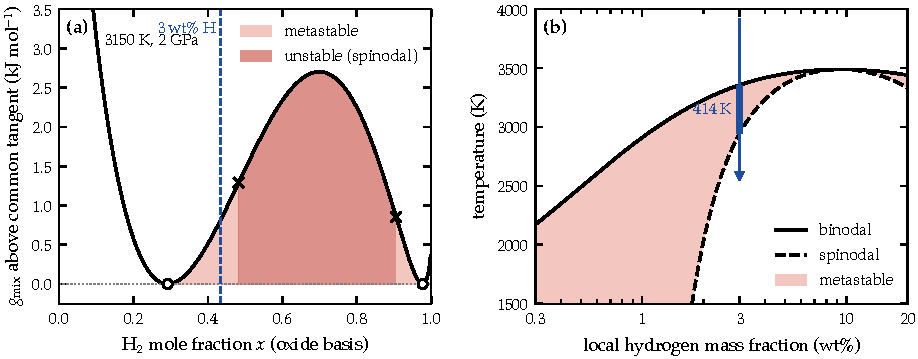
\includegraphics[width=\textwidth]{fig1_1_concept}
\thesiscaption{Binodal, spinodal and the metastable window of a cooling H$_2$--MgSiO$_3$
parcel.}{(a) Homogeneous Gibbs energy of mixing at 2\,GPa and 3150\,K above its common
tangent, for the published mixing model \cite{gilmore2026}. Circles mark the coexisting
compositions (binodal), crosses the inflection points (spinodal). A parcel with 3\,wt\%
local hydrogen (dashed line) is metastable here. (b) Binodal and spinodal temperatures at
2\,GPa as a function of local hydrogen mass fraction. A 3\,wt\% parcel cooling at fixed
pressure (arrow) enters the miscibility gap at the binodal but becomes unstable only at the
spinodal.}
\label{fig:concept}
\end{figure*}

The size of this window matters for sub-Neptunes, because it sets when, and at which
temperature, hydrogen leaves the interior. Delayed exsolution would release hydrogen later
and more abruptly. Through the atmospheric hydrogen budget, the timing of this release
feeds into the speciation equilibria that set the observable composition, such as the
H$_2$O/H$_2$ and CO$_2$/CH$_4$ ratios that we studied in our thesis \cite{laga2025}, and the
silane--methane competition proposed as a magma-ocean diagnostic \cite{hakim2026}. Whether
the window is large enough to matter has not been quantified.

The spinodal is a property of the homogeneous free energy inside the miscibility gap.
Simulations of coexisting phases constrain where the gap is, but not the free energy of the
homogeneous fluid within it. A spinodal derived from a fitted mixing model therefore
inherits the assumptions of its functional form. This makes \textbf{identifiability} the
central question of this work: how far do the existing data constrain the metastable free
energy, and with it the delay?

\section{Objectives and Scope}

This work investigates the thermodynamic limits on hydrogen exsolution from sub-Neptune
magma oceans using \Atm{}, a python-based modeling framework. We focus specifically on
closed H$_2$--MgSiO$_3$ parcels with local hydrogen mass fractions ranging from 0.1\% to 20\%,
at pressures of 2 to 10\,GPa, cooling through temperatures of 2,000 to 4,000\,K. These local
mass fractions describe the fluid at the magma-atmosphere boundary, not the hydrogen budget
of the whole planet.

The primary objectives of this work are to:
\begin{enumerate}
\item \textbf{Implement the final 2026 hydrogen--silicate mixing model} \cite{gilmore2026} in
\Atm{}, with a consistent conversion between the published oxide composition basis and the
native formula units of \Atm{}.
\item \textbf{Quantify the metastable window} between binodal and spinodal along cooling
paths, and the hydrogen inventory that delayed exsolution could withhold from separation.
\item \textbf{Audit the published fit against its source simulations}, and resolve the
mismatches that this audit reveals.
\item \textbf{Determine how well existing data constrain the metastable free energy}, by
recalibrating several smooth model classes against the same data, and identify the
simulations that would settle the question.
\end{enumerate}

This work is constrained to equilibrium thermodynamics and its local stability limits. We
acknowledge that real planets may exhibit nucleation on existing interfaces, finite cooling
rates, convective mixing and settling of the separated phases. We do not compute a
nucleation rate, a planetary radius or an atmospheric spectrum. However, establishing the
stability limits is essential: they bound the largest possible delay, define the boundary
conditions for kinetic models, and identify which measurements are needed before a kinetic
model can be trusted.

\chapter{Methodology}\label{ch:methodology}

This section outlines the complete modeling framework used to determine the equilibrium and
stability limits of hydrogen exsolution at the magma-atmosphere boundary of sub-Neptune
exoplanets, called the core--envelope boundary in \cite{gilmore2026}. The implementation is
performed using \Atm{} \cite{bower2025}, an open-source Python library designed to resolve
coupled chemical equilibrium and mass-balance constraints in gas-melt environments. In the
following sections, we outline the conceptual basis, numerical approach, chemical system,
and software validation.

\section{Formulation and Numerical Solution}

\subsection{Solver Architecture}

Users define the gaseous species, from which the software generates an independent reaction
basis using Gaussian elimination (Leal et al.\ 2016 \cite{leal2016}). At the interface, the
solver determines chemical equilibrium among gas species and any specified dissolved species
within the melt, subject to elemental mass conservation. The solver determines the
equilibrium state by minimizing the total Gibbs free energy using the optimistix framework,
with
\begin{equation}
G = \sum_i n_i \mu_i(T,P),
\label{eq:gibbs}
\end{equation}
where $n_i$ is the number of moles and $\mu_i$ is the chemical potential of species $i$,
which includes EOS corrections and melt interactions. \Atm{} employs the extended law of mass
action (xLMA; Leal et al.\ 2016 \cite{leal2016}) to build a closed nonlinear system that
integrates equilibrium chemistry with elemental mass balance, structured as a root-finding
problem, and leverages JAX for high-performance computations (Bradbury et al.\ 2018
\cite{jax2018}). The nonlinear system is resolved using robust Newton--type root--finders
augmented with line--search and trust--region safeguards.

For this work we extended the phase-equilibrium module of \Atm{}. A binary mixing model now
supplies the nonideal activities of two condensed components, here MgSiO$_3$ and H$_2$. The
same Gibbs energy yields the homogeneous activities, the coexisting compositions, the local
stability and the equilibrium (convex-envelope) free energy, so that all quantities in this
work follow from one function.

\subsection{Phase Equilibrium and Local Stability}

For a binary mixture with molar Gibbs energy of mixing $g_{\rm mix}(x)$, two phases $\alpha$
and $\beta$ coexist when both component chemical potentials are equal,
\begin{equation}
\mu_{\rm sil}^{\alpha} = \mu_{\rm sil}^{\beta},\qquad
\mu_{\rm H_2}^{\alpha} = \mu_{\rm H_2}^{\beta},
\label{eq:coexistence}
\end{equation}
which is the common-tangent construction. The locus of coexisting compositions as a function
of temperature is the \textbf{binodal}. A homogeneous mixture is locally stable as long as
\begin{equation}
\frac{\partial^2 g_{\rm mix}}{\partial x^2} > 0,
\label{eq:stability}
\end{equation}
and the locus where this curvature vanishes is the \textbf{spinodal}. Between the binodal and
the spinodal a homogeneous mixture is metastable: it is stable against small composition
fluctuations, but a nucleus of the other phase that exceeds a critical size lowers the free
energy \cite{debenedetti1996}. Inside the spinodal it decomposes spontaneously
\cite{cahn1961}. Both conditions are evaluated with bracketed root finding on the two stable
branches, which excludes the trivial equal-composition solution, and with implicit
derivatives for use inside the \Atm{} solver.

\section{Hydrogen--Silicate Mixing Model}\label{sec:mixing_model}

Gilmore \& Stixrude \cite{gilmore2026} describe their phase-coexistence and homogeneous
DFT-MD simulations with an asymmetric regular solution model. We write their equation~8 as
\begin{equation}
\begin{split}
g_{\rm mix} ={}& W(x)\left(1-\frac{T}{\tau}+\frac{P}{\pi}\right)\\
 &+ RT\left[x\ln x + (1-x)\ln(1-x)\right],
\end{split}
\label{eq:gs26}
\end{equation}
with the excess enthalpy at zero pressure
\begin{equation}
W(x) = x(1-x)\left[A(1-x)+Bx\right],
\label{eq:w}
\end{equation}
excess entropy $W/\tau$ and excess volume $W/\pi$. The published parameters are
$A = 75$\,kJ\,mol$^{-1}$, $B = 424$\,kJ\,mol$^{-1}$, $\tau = 4{,}400$\,K and
$\pi = -35$\,GPa. The composition variable is the molar fraction of the H$_2$ component on an
oxide basis,
\begin{equation}
\begin{split}
x &= \frac{N_{\rm H_2}}{N_{\rm H_2}+N_{\rm MgO}+N_{\rm SiO_2}}\\
  &= \frac{N_{\rm H}/2}{N_{\rm H}/2 + 2(N_{\rm Mg}+N_{\rm Si}+N_{\rm O})/5}.
\end{split}
\label{eq:x}
\end{equation}
The paper does not state which component carries $A$ and which carries $B$. The critical
temperature is the same for both choices, but the shape of the miscibility gap is not.
Assigning $B$ to the H$_2$-rich side (Eq.~\ref{eq:w}) reproduces the published curves of
their Figure~2 and their statement that the hydrogen-poor phase holds more hydrogen than the
hydrogen-rich phase holds silicate (Section~\ref{sec:verification}).

\paragraph{Composition basis.} \Atm{} uses native formula units, with the H$_2$ fraction
$y = n_{\rm H_2}/(n_{\rm H_2}+n_{\rm MgSiO_3})$. One MgSiO$_3$ unit contains two oxide units,
so
\begin{equation}
x = \frac{y}{2-y}, \qquad
G = \left(2\,n_{\rm MgSiO_3} + n_{\rm H_2}\right) g_{\rm mix}(x).
\label{eq:basis}
\end{equation}
The second relation keeps the free energy extensive; the native chemical potentials are
$\mu_{\rm MgSiO_3} = 2\mu_{\rm oxide}$ and $\mu_{\rm H_2}$. Converting only the endpoint
compositions is not sufficient, because the native curvature, activities and phase amounts
all depend on the factor $2-y$. We implemented this conversion as a static multiplicity of
the silicate component, available through the constructor
\texttt{hydrogen\_silicate\_gilmore26} of the class \texttt{SubregularSolution}.

\paragraph{Controls.} As controls we retain the historical 2025 parameterization of Rogers,
Young \& Schlichting \cite{rogers2025} on its own formula-unit basis, and a deliberately
incorrect import of the 2026 parameters without the basis conversion. The latter is a
diagnostic, never a recommended model.

\section{Delayed-Exsolution Limit}\label{sec:delayed}

We follow a closed, initially homogeneous parcel that cools at fixed pressure. Its local
hydrogen mass fraction $w$ fixes $y$ and hence $x$. On cooling it first enters the
miscibility gap at the binodal temperature $T_b(w,P)$ and later becomes locally unstable at
the spinodal temperature $T_{\rm sp}(w,P)$. Because Eq.~(\ref{eq:gs26}) is linear in $T$,
the spinodal temperature follows analytically from Eq.~(\ref{eq:stability}):
\begin{equation}
T_{\rm sp} = \frac{-W''(x)\,(1+P/\pi)}{R/[x(1-x)] - W''(x)/\tau}.
\label{eq:tsp}
\end{equation}
We compare two limiting histories. In the \textbf{equilibrium limit} the parcel separates as
soon as it crosses $T_b$. In the \textbf{delayed limit} nucleation is suppressed until
$T_{\rm sp}$, after which the parcel equilibrates rapidly. We report the metastable interval
\begin{equation}
\Delta T_{\rm ms} = T_b - T_{\rm sp},
\label{eq:interval}
\end{equation}
and the fraction of all hydrogen that the equilibrium limit already places in the H-rich
phase at $T_{\rm sp}$,
\begin{equation}
f_{\rm H} = \frac{\phi\, y_{\rm rich}}{y_0}, \qquad
\phi = \frac{y_0-y_{\rm poor}}{y_{\rm rich}-y_{\rm poor}},
\label{eq:fh}
\end{equation}
where $\phi$ is the native mole fraction of the H-rich phase from the lever rule. The quantity
$f_{\rm H}$ is the largest inventory that the delayed limit can withhold from separation. It is
a bound between two assumptions, not a computed release rate: both histories conserve all
hydrogen, and the delayed parcel still holds its hydrogen dissolved in the silicate.

\section{Model Configurations and Parameter Space}

The results presented in the Results are derived from sweeps over four parameters. When
varying a specific parameter, the other three are held at their baseline values unless
otherwise noted.
\begin{enumerate}
\item \textbf{Local Hydrogen Mass Fraction (0.1\% -- 20\%):} This range spans parcels from
silicate-rich melt to hydrogen-rich fluid at the magma-atmosphere boundary.\\
\textit{Baseline:} $w = 3$\,wt\%, a composition that crosses both the binodal and the
spinodal above 2,000\,K.
\item \textbf{Pressure (2 -- 10\,GPa):} This range covers most of the magma-atmosphere
boundary pressures of the sub-Neptune models compiled in \cite{gilmore2026}.\\
\textit{Baseline:} $P = 2$\,GPa, the pressure of the best-sampled simulations.
\item \textbf{Temperature (2,000\,K -- 4,000\,K):} This window covers the fluid regime of the
simulations. We report spinodals below 2,000\,K separately and test stopping temperatures of
2,500 and 3,000\,K, because neither is a computed melting boundary.
\item \textbf{Mixing Model:} the published 2026 fit (baseline), the historical 2025 fit and
the incorrect-basis control, and the recalibrated model classes of
Section~\ref{sec:recalibration}.
\end{enumerate}
In total the onset grid contains \nOnsetRows{} rows and the cooling paths \nCoolingRows{}
states. A further \nStressRows{} deterministic stress cases change $A$, $B$, $\tau$ and
$|\pi|$ by $\pm10\%$, individually and in combination. These stress cases are not calibrated
uncertainties; Section~\ref{sec:recalibration} replaces them with data-driven posteriors.

\section{Source-Data Audit and Recalibration}\label{sec:recalibration}

\subsection{Source Data}

The source simulations are public \cite{gilmore2026data}. Extended Data (ED) Table~1 lists
14 phase-coexistence runs: four that kept two phases, with the composition of each phase, and
ten that became one homogeneous phase, with their bulk composition. The quoted composition
uncertainty is $\pm0.05$ in $x$. ED Table~2 lists homogeneous simulations at 5\,GPa and
4,000\,K: three mixtures and the two endmembers, with enthalpy, entropy and volume per atom.
We reconstruct excess properties per mole of mixing units (Eq.~\ref{eq:x}) and remove the
ideal mixing entropy from the total entropy. The endmember errors are shared between the
three mixtures, so we propagate a full covariance matrix. The endmembers were simulated at
5.00\,GPa and the mixtures at 5.06--5.08\,GPa; we add the corresponding enthalpy and volume
shifts as a fully correlated systematic error. Finally, we digitized the published
Figure~2a, which shows the same coexistence runs, from the CC-BY figure file.

\subsection{Likelihood and Model Classes}

We compare models with the data through three terms,
\begin{equation}
\chi^2 = \chi^2_{\rm phase} + \chi^2_{\rm comp} + \chi^2_{\rm hom}.
\label{eq:chi2}
\end{equation}
The first term uses the most robust information in the source: whether each of the 14 runs
kept one or two phases. A model that misplaces a run pays
$[(T_{\rm run}-T_b)/\sigma_T]^2$, with $T_b$ the model binodal temperature at the run's bulk
composition and $\sigma_T^2 = (50\,{\rm K})^2 + (100\,{\rm K\,GPa^{-1}}\,\sigma_P)^2$, which
adds the quoted pressure error. The second term compares the eight coexisting compositions,
with the quoted $\pm0.05$ treated as a Gaussian standard deviation. The third term compares
the nine homogeneous excess properties with their covariance.

We fit four smooth model classes with constant excess enthalpy, entropy and volume, so that
their spinodals follow in closed form. They are written as Redlich--Kister series
\cite{redlich1948},
\begin{equation}
G_{\rm ex} = \sum_k \left(h_k - T s_k + P v_k\right) x(1-x)(1-2x)^k,
\label{eq:rk}
\end{equation}
summarized in Table~\ref{tab:classes}. Class M1 is the published form. M2 frees the shapes
of the excess entropy and volume. M3 and M4 add one and two higher composition terms that
share the published temperature and pressure scaling.

\begin{table}[t]
\thesiscaption{Model classes used in the recalibration.}{All classes have constant excess
enthalpy, entropy and volume coefficients. The last column counts free parameters.}
\label{tab:classes}
\small\centering
\begin{tabular}{@{}llc@{}}
\toprule
Class & Excess Gibbs energy & $n$\\
\midrule
M1 & published form, Eq.~(\ref{eq:gs26}) & 4\\
M2 & subregular $H$, $S$ and $V$, independent & 6\\
M3 & RK order 2, published $T,P$ scaling & 5\\
M4 & RK order 3, published $T,P$ scaling & 6\\
\bottomrule
\end{tabular}
\end{table}

Priors are uniform within broad stated bounds; we sample $1/\tau$ and $1/\pi$ rather than
$\tau$ and $\pi$. We draw posterior samples with an adaptive Metropolis algorithm
\cite{haario2001}: eight chains of 12,000 steps, of which the first 3,000 adapt the proposal
and are discarded. We check convergence with the split-chain $\hat R$ statistic
\cite{gelman2013}. Besides the full data set we fit five variants of class M1: with the
Figure~2a compositions, with $\sigma_x = 0.15$ for the two runs closest to $T_C$, without
the excess volumes, and with only the phase states plus either the compositions or the
homogeneous data. For every retained sample we recompute $T_b$, $T_{\rm sp}$,
$\Delta T_{\rm ms}$, $f_{\rm H}$ and $T_C$ at the baseline.

\subsection{Identifiability Test}

To test whether coexistence data can identify the spinodal at all, we add a nonnegative
perturbation that lives only inside the miscibility gap,
\begin{equation}
\delta g = 64\,\lambda B_{\rm gap}\, u^3(1-u)^3,\quad
u = \frac{x-x_{\rm poor}}{x_{\rm rich}-x_{\rm poor}},
\label{eq:bump}
\end{equation}
for $x_{\rm poor}<x<x_{\rm rich}$ and zero elsewhere. Here $B_{\rm gap}$ is the height of the
published free energy above its common tangent at the middle of the gap. The perturbation and
its first two derivatives vanish at the binodal, so all coexisting compositions, all
equilibrium free energies and all homogeneous states outside the gap stay exactly the same.
The amplitudes $\lambda = 0$ to 8 are a counterexample to uniqueness, not a material model.

\section{Verification of Thermodynamic Consistency}\label{sec:verification}

We verified the implementation in three independent ways. First, our implementation
reproduces the published model. Its critical temperatures are \pubTcTwo{}\,K at 2\,GPa and
\pubTcTen{}\,K at 10\,GPa, matching the published 3,500 and 2,600\,K, and our binodals follow
the digitized curves of the published Figure~2a with an RMS residual of at most \digRms{}\,K
(Figure~\ref{fig:verification}a). The largest single deviation, \digMax{}\,K, is about three
pixels of the printed line.

Second, a separate scalar implementation, written without any code from \Atm{}, agrees with
the \Atm{} binodal and spinodal temperatures to within \indepMaxDiff{}\,K over the grid
(Figure~\ref{fig:verification}b). The exception is the binodal within 0.02 of $x_C$, where the
flat crest makes the binodal temperature ill-conditioned and the two codes differ by up to
\indepMaxDiffCrit{}\,K. It locates spinodal compositions as the real roots of a
polynomial and binodals by nested bracketed root finding, so its errors are independent of
the \Atm{} solver.

Third, the \Atm{} test suite passed \nTests{} tests, including the extensive-energy
derivative test of the basis conversion (Eq.~\ref{eq:basis}), Gibbs--Duhem consistency and
spinodal temperatures against independent roots. The study itself checks conservation of
each native component in \nNativeSolves{} native equilibrium solves and compares 30 spinodal
temperatures with independent SciPy roots. The largest elemental and lever-rule errors are
$2.2\times10^{-16}$.

\begin{figure*}[t]
\centering
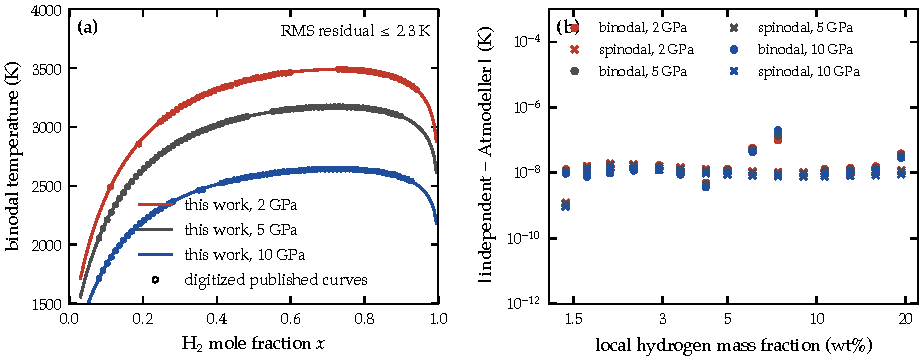
\includegraphics[width=\textwidth]{fig2_1_verification}
\thesiscaption{Internal consistency check of \Atm{}.}{(a) Binodal temperatures of our
implementation of Eq.~(\ref{eq:gs26}) (lines) and the curves digitized from Figure~2a of
\cite{gilmore2026} (circles) at 2, 5 and 10\,GPa. (b) Absolute difference between a separate
scalar implementation and \Atm{} for the binodal (circles) and spinodal (crosses)
temperatures across the onset grid. The two codes share no solver code.}
\label{fig:verification}
\end{figure*}

\section{Data Processing, Model Limitations and Assumptions}

\subsection{Data Processing}

Model outputs were exported as CSV and JSON files with SHA-256 hashes of every artifact and
analysis script. Data reduction was performed using pandas, and visualizations were generated
using matplotlib. Key diagnostics reported in the Results include the binodal and spinodal
temperatures, the metastable interval $\Delta T_{\rm ms}$, the withheld hydrogen fraction
$f_{\rm H}$ and the critical temperature $T_C$.

\subsection{Model Limitations and Assumptions}

The current framework operates under several constraints. First, the mixture is a binary
H$_2$--MgSiO$_3$ system; helium, iron and other volatiles are absent, and the source
simulations used pure MgSiO$_3$. Second, all model classes have constant excess enthalpy,
entropy and volume, so the free energy is linear in temperature and pressure. Third, the
local mass fractions describe a closed parcel; we do not model transport between the
interior and the envelope, convection or settling. Finally, the approach treats nucleation
only as two limiting cases, neglecting nucleation rates, interfacial energies,
diffusion-limited growth and spatial gradients within the reservoirs.

\chapter{Results}\label{ch:results}

This chapter details the equilibrium and stability limits of hydrogen exsolution from
H$_2$--MgSiO$_3$ mixtures. We begin by characterizing the binodal and spinodal of the
published mixing model across pressure and composition, establishing the metastable window.
Building on this, we analyze the hydrogen inventory that delayed exsolution could withhold
along cooling paths. Subsequently, the published fit is audited against its source
simulations and recalibrated against the same data. The chapter concludes with a test of
whether coexistence data can identify the spinodal at all.

\section{Phase Boundaries and the Metastable Window}\label{sec:window}

Figure~\ref{fig:phase_maps} shows the binodal and spinodal temperatures of the published
model as a function of local hydrogen mass fraction at 2, 5 and 10\,GPa. The binodal is
flat-topped: its crest at 2\,GPa lies at $T_C = \pubTcTwo{}$\,K and $x_C = \pubXc{}$
($w = \pubWc{}$\,wt\%), and it falls only slowly away from $x_C$. The spinodal touches the
binodal at the critical point and falls steeply on the hydrogen-poor side. Spinodals exist
only above $w = \pubThreshold{}$\,wt\%. Below this threshold a parcel can still separate in
equilibrium, but its homogeneous state never becomes unstable, so separation always requires
nucleation (Appendix~\ref{app:thermo}).

\begin{figure}[t]
\centering
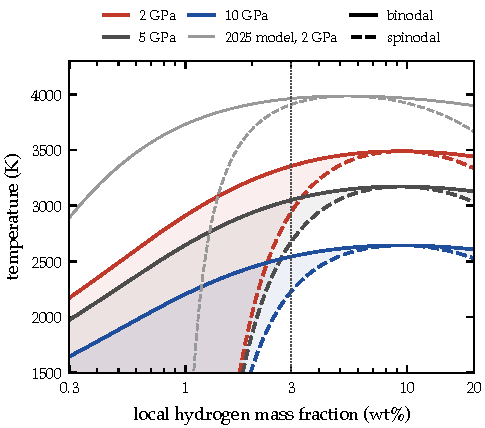
\includegraphics[width=\columnwidth]{fig3_1_phase_maps}
\thesiscaption{Binodal and spinodal temperatures of the published mixing model.}{Solid
lines show the binodal, dashed lines the spinodal, at 2, 5 and 10\,GPa; shading marks the
metastable window. Grey lines show the historical 2025 parameterization at 2\,GPa. The dotted
line marks the 3\,wt\% baseline.}
\label{fig:phase_maps}
\end{figure}

For the baseline parcel of 3\,wt\% hydrogen at 2\,GPa, the binodal lies at \pubTbTwo{}\,K and
the spinodal at \pubTspTwo{}\,K. The metastable interval is therefore \pubIntTwo{}\,K
(Table~\ref{tab:onsets}). It shrinks to \pubIntFive{}\,K at 5\,GPa and \pubIntTen{}\,K at
10\,GPa, because both onset temperatures scale with $1+P/\pi$. At 10\,GPa the spinodal lies
below the coldest two-phase simulation (2,500\,K), so it is an extrapolation.

\begin{table}[t]
\thesiscaption{Onset temperatures for a parcel with 3\,wt\% local hydrogen.}{$f_{\rm H}$ is
the fraction of hydrogen that equilibrium places in the H-rich phase at the spinodal.}
\label{tab:onsets}
\small\centering
\setlength{\tabcolsep}{4.5pt}
\begin{tabular}{@{}lrrrr@{}}
\toprule
Model, $P$ & $T_b$ (K) & $T_{\rm sp}$ (K) & $\Delta T_{\rm ms}$ (K) & $f_{\rm H}$ (\%)\\
\midrule
2026 fit, 2\,GPa & \pubTbTwo & \pubTspTwo & \pubIntTwo & \pubFhTwo\\
2026 fit, 5\,GPa & \pubTbFive & \pubTspFive & \pubIntFive & \pubFhFive\\
2026 fit, 10\,GPa & \pubTbTen & \pubTspTen & \pubIntTen & \pubFhTen\\
2025 fit, 2\,GPa & \oldTbTwo & \oldTspTwo & \oldIntTwo & \oldFhTwo\\
Wrong basis, 2\,GPa & \wrongTbTwo & \wrongTspTwo & \wrongIntTwo & \wrongFhTwo\\
\bottomrule
\end{tabular}
\end{table}

The composition basis matters. The historical 2025 parameterization gives an interval of only
\oldIntTwo{}\,K, and importing the 2026 parameters without the basis conversion gives
\wrongIntTwo{}\,K. With the correct conversion the interval is about nine times larger.
Changing $A$, $B$, $\tau$ and $|\pi|$ by $\pm10\%$ gives intervals of
\stressIntLo{}--\stressIntHi{}\,K. These stress cases are not calibrated uncertainties;
Section~\ref{sec:recalibrated} derives uncertainties from the data.

\section{Hydrogen Inventory along Cooling Paths}\label{sec:inventory}

Figure~\ref{fig:inventory}a follows the 3\,wt\% parcel as it cools. In the equilibrium limit
the H-rich phase appears at $T_b$ and grows on further cooling. In the delayed limit nothing
separates until $T_{\rm sp}$, where the parcel jumps to the equilibrium state. At the spinodal
the equilibrium limit already places \pubFhTwo{}\% of all hydrogen in the H-rich phase, while
the delayed limit still holds it in the homogeneous parcel.

\begin{figure}[t]
\centering
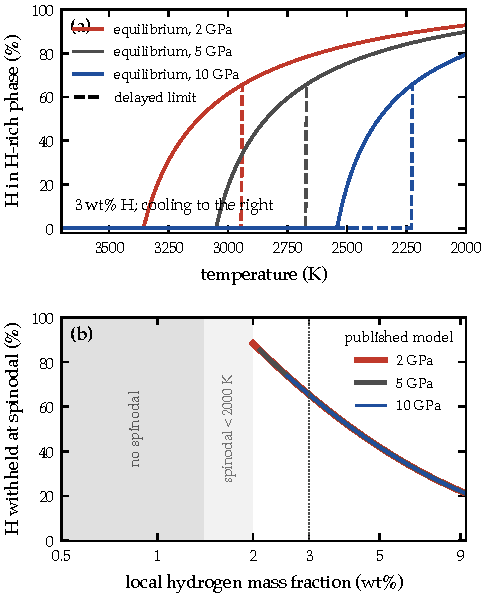
\includegraphics[width=\columnwidth]{fig3_2_inventory}
\thesiscaption{Hydrogen withheld by delayed exsolution.}{(a) Fraction of all hydrogen in
the H-rich phase for a 3\,wt\% parcel cooling at 2, 5 and 10\,GPa, in the equilibrium limit
(solid) and the delayed limit (dashed). (b) Fraction withheld at the spinodal as a function of
local hydrogen mass fraction. The curves for the three pressures coincide.}
\label{fig:inventory}
\end{figure}

At 3,000\,K and 2\,GPa the baseline parcel is metastable. Equilibrium would place
\eqFhThreeThousand{}\% of its hydrogen in the H-rich phase, which is \gramsWithheld{}\,g of the
30\,g of hydrogen in each kilogram of parcel, whereas the delayed limit has not separated at
all. Equilibration would lower the Gibbs energy by \energyLowering{}\,kJ per native mole. This
is a free-energy difference, not a prediction of released heat.

The withheld fraction at the spinodal is the same at 2, 5 and 10\,GPa to within
\fhPressureSpread{}, or \fhPressureSpreadAll{} within 0.1\,wt\% of the critical composition,
where the lever rule becomes ill-conditioned (Figure~\ref{fig:inventory}b). It falls from 88\%
at 2\,wt\%, the lowest composition whose spinodal lies above 2,000\,K, to about 21\% near the
critical composition. The pressure invariance
follows from the separable form of Eq.~(\ref{eq:gs26}) (Appendix~\ref{app:thermo}); it is not
independent evidence.

\section{Audit of the Published Fit against its Source Data}\label{sec:audit}

Our implementation reproduces the published model (Section~\ref{sec:verification}), so any
mismatch with the source simulations belongs to the published fit itself. The fit agrees with
all ten one-phase runs. For the two-phase run at 1.65\,GPa, its gap at 3,500\,K lies entirely
above the bulk composition of the cell, a miss of \pubMissOneSixFive{}\,K in temperature.
It reproduces both compositions within the quoted $\pm0.05$ for only one of the four
two-phase runs (Table~\ref{tab:ed1}, Figure~\ref{fig:audit}b).

\begin{figure*}[t]
\centering
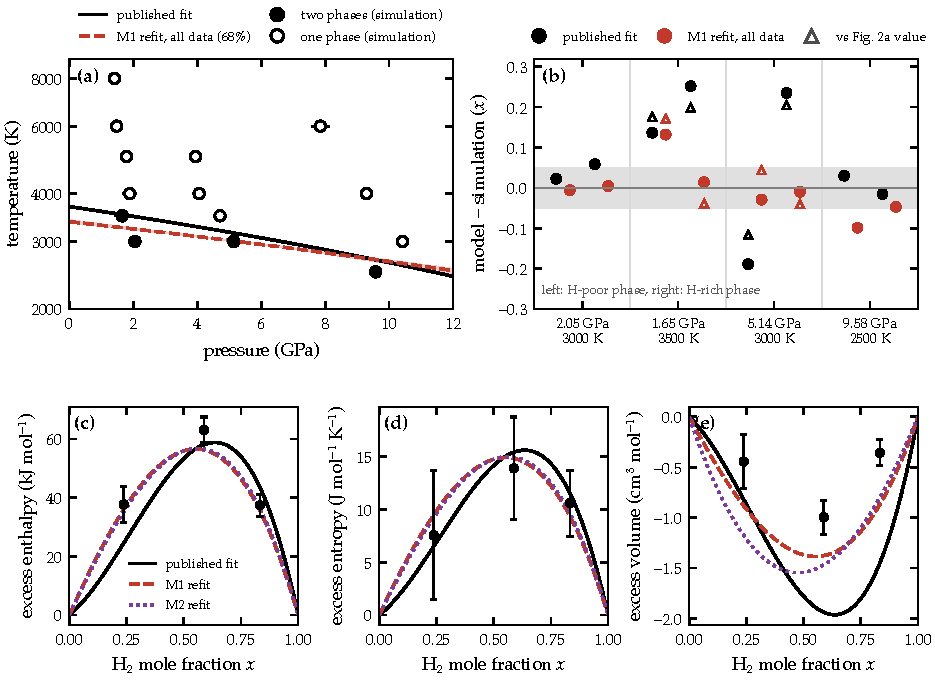
\includegraphics[width=\textwidth]{fig3_3_source_audit}
\thesiscaption{Audit of the published fit against its source simulations.}{(a) Phase state of
the 14 coexistence runs (filled: two phases; open: one phase) with the published critical
curve (black) and the critical curve of the refit to all data (red, 68\% band). (b) Model
minus simulation for the eight coexisting compositions, against ED Table~1 (circles) and the
digitized Figure~2a (triangles); the grey band is the quoted $\pm0.05$. (c--e) Excess
enthalpy, entropy and volume of the homogeneous simulations at 5\,GPa and 4,000\,K
(symbols, 1$\sigma$), with the published fit and the refits of classes M1 and M2.}
\label{fig:audit}
\end{figure*}

\paragraph{Near-critical runs.} The largest misses occur for the two runs closest to the
critical curve. The published $T_C$ lies \tcAboveRunNearCritLow{}\,K above the run at
1.65\,GPa and 3,500\,K, and \tcAboveRunNearCritHigh{}\,K above the run at 5.14\,GPa and
3,000\,K. For the first run the model predicts a gap centred at $x \approx 0.71$, whereas the
simulation shows a gap centred at 0.52. For exactly these two runs the source table and the
source figure disagree. The digitized Figure~2a places the pairs at
(\figLoOneSixFive{}, \figHiOneSixFive{}) and (\figLoFiveOneFour{}, \figHiFiveOneFour{}),
whereas ED Table~1 lists (0.458, 0.576) and (0.587, 0.706). The differences range from
\diffLoFiveOneFour{} to \diffHiOneSixFive{}. For the two wide-gap runs, table and figure agree
to within \digMarker{}.

In all four two-phase runs, the per-phase atom numbers in ED Table~1 add up to the full
simulation cell, so every interfacial atom is counted in one of the two phases. With sharp
interfaces this matters little. Near $T_C$, however, interfaces broaden, and such a count
pulls both compositions toward the bulk composition of the cell, which is 0.526 and 0.629 for
these runs. The two composition estimators described in the source methods
\cite{gilmore2026} could therefore differ most for exactly these runs, as observed. We treat
the near-critical compositions as uncertain at the 0.04--0.07 level. This is an inference from
the published numbers, not a demonstrated cause.

\paragraph{Homogeneous simulations.} The homogeneous simulations reveal a second mismatch
(Figure~\ref{fig:audit}c--e). The published fit predicts an excess volume of
$\vModMid$\,cm$^3$\,mol$^{-1}$ at $x = \xMid{}$, whereas the simulations give
$\vObsMid \pm \vSigMid$\,cm$^3$\,mol$^{-1}$. Because the excess volume sets the pressure dependence of $T_C$,
the value $\pi = -35$\,GPa reproduces the critical curve between 2 and 10\,GPa, but the
directly simulated volumes imply a pressure scale about twice as large in magnitude. The fit
also underestimates the excess enthalpy at $x = 0.24$. In total, the published fit has
$\chi^2 = \pubChiPhase{}$ for the 14 phase states, \pubChiComp{} for the eight compositions
and \pubChiHom{} for the nine homogeneous properties.

These comparisons reproduce checks against the data from which the fit was built. They are
not independent validation, and they do not show that any simulation is wrong. They show
that one four-parameter model cannot follow all of the source data at once.

\section{Recalibrated Delayed-Exsolution Interval}\label{sec:recalibrated}

Table~\ref{tab:recalibration} and Figure~\ref{fig:posteriors} summarize the nine refits.
Refitting the published form (class M1) to all data lowers $\chi^2$ from \pubChiTotal{} to
\ChiMOneTable{}. The best fit is much less asymmetric than the published one
(Table~\ref{tab:map}) and has a lower critical temperature,
$T_C(2\,{\rm GPa}) = \TcMOneTable{}$\,K (68\% range \TcMOneTableLo{}--\TcMOneTableHi{}\,K). It
pays for this with the phase state of the run at 1.65\,GPa and 3,500\,K, which it places
\MissMOneTable{}\,K above its binodal. The metastable interval of the baseline parcel shrinks
to \IntMOneTable{}\,K (\IntMOneTableLo{}--\IntMOneTableHi{}\,K), and the withheld fraction to
\FhMOneTable{}\%.

\begin{table*}[t]
\thesiscaption{Recalibration of the hydrogen--silicate mixing model.}{$\chi^2$ terms at the
best fit for the 14 phase states, the 8 compositions and the 9 homogeneous properties, and
posterior medians with 68\% ranges of the critical temperature at 2\,GPa, the metastable
interval and the withheld hydrogen fraction for a 3\,wt\% parcel at 2\,GPa. Fits marked
$\dagger$ leave out data (dashes), so their $\chi^2$ cannot be compared with the others.}
\label{tab:recalibration}
\small\centering
\begin{tabular}{@{}lrrrlll@{}}
\toprule
Fit & $\chi^2_{\rm phase}$ & $\chi^2_{\rm comp}$ & $\chi^2_{\rm hom}$ & $T_C$ (K) &
$\Delta T_{\rm ms}$ (K) & $f_{\rm H}$ (\%)\\
\midrule
\inputtable{tables/recalibration.tex}
\bottomrule
\end{tabular}
\end{table*}

\begin{figure*}[t]
\centering
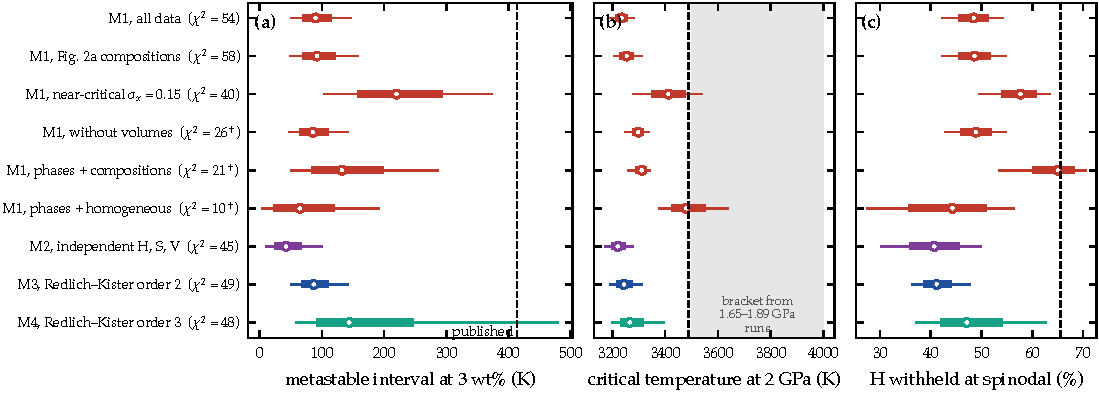
\includegraphics[width=\textwidth]{fig3_4_posteriors}
\thesiscaption{Posterior distributions of the delayed-exsolution quantities.}{(a) Metastable
interval, (b) critical temperature at 2\,GPa and (c) withheld hydrogen fraction for a 3\,wt\%
parcel at 2\,GPa, for each model class and data treatment. Thick bars show 68\% and thin bars
95\% intervals; open circles mark medians. Dashed lines mark the published fit; the grey band
in (b) is the bracket set by the two-phase run at 1.65\,GPa and the one-phase run at
1.89\,GPa, drawn without correction to 2\,GPa. Labels give the best-fit $\chi^2$; fits marked
$\dagger$ use fewer data.}
\label{fig:posteriors}
\end{figure*}

The data treatments show which data drive this shift (Table~\ref{tab:map}). Without the
homogeneous data, the fit returns to the published asymmetry, $B/A = \BAMOnePhaseComp{}$
against 5.65, but with interaction parameters three times larger and a lower $\tau$. Its
interval is \IntMOnePhaseComp{}\,K, not \pubIntTwo{}\,K, so the asymmetry alone does not set the
interval: the excess entropy and the strength of the interaction matter as much. With the
homogeneous data but without the compositions, the excess is nearly symmetric,
$B/A = \BAMOnePhaseHom{}$, and the interval is \IntMOnePhaseHom{}\,K. The compositions themselves
discriminate weakly between these fits: their misfit is $\chi^2_{\rm comp} =
\ChiCompMOnePhaseComp{}$ for the strongly and \ChiCompMOneTable{} for the weakly asymmetric
fit. The difference lies mainly in the phase states and the
homogeneous data. Using the Figure~2a compositions instead of ED Table~1 gives
\IntMOneFigure{}\,K, and dropping the excess volumes gives \IntMOneNoVolume{}\,K: the volume
mismatch controls the pressure dependence of $T_C$, but hardly the interval at 2\,GPa. Giving
the two near-critical runs a composition uncertainty of 0.15 raises the asymmetry to
$B/A = \BAMOneInflated{}$ and lengthens the interval to \IntMOneInflated{}\,K.

Every refit that uses the coexisting compositions places the run at 1.65\,GPa and 3,500\,K
between \missLo{} and \missHi{}\,K above its binodal. This reflects a tension within the source
data. The narrow gap at 5.14\,GPa and 3,000\,K requires $T_C$ close to 3,000\,K at that pressure,
whereas the two-phase state at 1.65\,GPa requires $T_C > 3{,}500$\,K. A linear critical curve
meets both only if it falls by more than about \slopeMinimum{}\,K per GPa. The published fit falls
by \slopePublished{}\,K per GPa, and the fit to phase states and homogeneous data by
\SlopeMOnePhaseHom{}\,K per GPa.

The more flexible classes fit the data with $\chi^2 = \ChiMTwo{}$ (M2), \ChiMThree{} (M3) and
\ChiMFour{} (M4), against \ChiMOneTable{} for M1. Their intervals are \IntMTwo{},
\IntMThree{} and \IntMFour{}\,K. None of the classes fits all data within the quoted errors: for 31 data
points, $\chi^2$ stays between \ChiMTwo{} and \ChiMOneTable{}. Across all nine refits the median
interval ranges from \IntRangeLo{} to \IntRangeHi{}\,K, compared with \pubIntTwo{}\,K for the
published fit (Table~\ref{tab:recalibration}, Figure~\ref{fig:posteriors}a). The most flexible class, M4, does not
exclude the published value: its 95\% range is \IntMFourLoNinetyFive{}--\IntMFourHiNinetyFive{}\,K. Every fit met our convergence criterion of a
split-chain $\hat R < 1.1$; the largest value is \maxRhat{}.

\begin{figure*}[t]
\centering
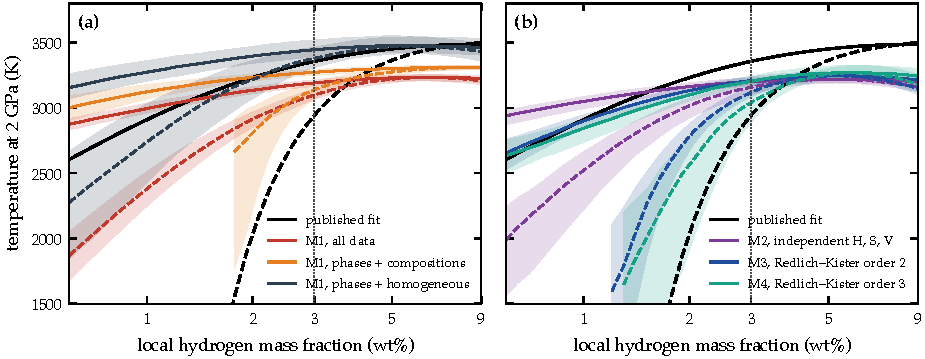
\includegraphics[width=\textwidth]{fig3_5_posterior_phase_diagrams}
\thesiscaption{Posterior binodals and spinodals at 2\,GPa.}{Medians (lines) and 68\% bands of
the binodal (solid) and spinodal (dashed) for (a) class M1 with three data treatments and (b)
classes M2--M4 with all data, compared with the published fit (black).}
\label{fig:posterior_diagrams}
\end{figure*}

\section{Identifiability of the Spinodal}\label{sec:identifiability}

The perturbation of Eq.~(\ref{eq:bump}) leaves the binodal, the equilibrium free energy and
every homogeneous state outside the gap unchanged; we verified this to within
$4\times10^{-12}$\,J\,mol$^{-1}$. It nevertheless moves the spinodal
(Figure~\ref{fig:identifiability}). At $\lambda = 8$ the 3\,wt\% spinodal rises by
\bumpThree{}\,K, the 5\,wt\% spinodal falls by \bumpFiveAbs{}\,K and the 2\,wt\% spinodal rises by
\bumpTwo{}\,K. Coexistence data alone therefore cannot identify the spinodal. Any spinodal
inferred from them is a property of the assumed functional form.

\begin{figure*}[t]
\centering
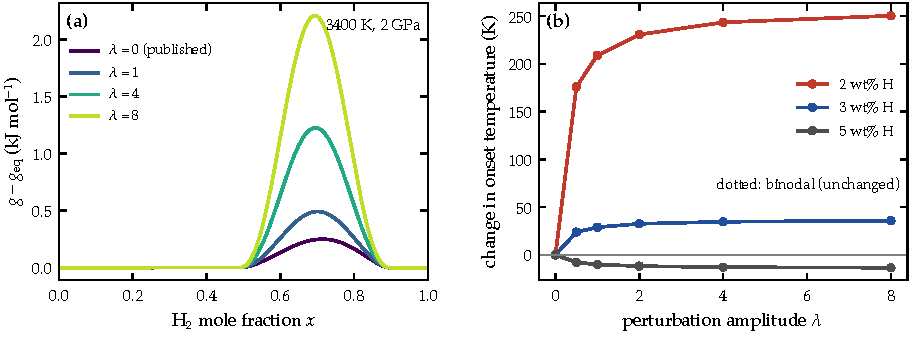
\includegraphics[width=\textwidth]{fig3_6_identifiability}
\thesiscaption{Two free energies with the same equilibrium but different spinodals.}{(a)
Homogeneous Gibbs energy above the equilibrium (convex-envelope) free energy at 3,400\,K and
2\,GPa for perturbation amplitudes $\lambda$ = 0 to 8. Outside the gap all curves are zero.
(b) Change of the spinodal (solid) and binodal (dotted) temperatures with $\lambda$ for 2, 3
and 5\,wt\% local hydrogen.}
\label{fig:identifiability}
\end{figure*}

\chapter{Discussion}\label{ch:discussion}

The Results reveal that the onset of hydrogen exsolution from a sub-Neptune magma ocean
cannot be read from equilibrium miscibility data alone. The published mixing model predicts
a metastable window of several hundred kelvin, but the same source data, fitted with the
same or slightly more flexible forms, favour windows two to ten times shorter. In this
chapter, we interpret the physical mechanisms behind these results and discuss how they
bear on the evolution and observable properties of sub-Neptune exoplanets.

\section{Why Equilibrium Data Cannot Fix the Spinodal}\label{sec:why}

The binodal and the spinodal probe different parts of the free energy. The binodal follows
from the common tangent, so it depends only on the free energy at the two coexisting
compositions and on the line between them. The spinodal depends on the local curvature of
the homogeneous free energy between those compositions, where a phase-separated simulation
never samples the homogeneous state. The perturbation of Section~\ref{sec:identifiability}
makes this explicit: it changes the curvature inside the gap and leaves every equilibrium
observable unchanged.

Fitting a smooth model with few parameters ties the curvature inside the gap to the free
energy outside it. The spinodal is then exactly as well constrained as these parameters. For
the baseline parcel three of them matter together: the asymmetry $B/A$, which sets the critical
composition, the excess entropy, set by $\tau$, and the strength of the interaction. The source
data pull them in different directions. Without the homogeneous data, the fit returns to the
published asymmetry ($B/A = \BAMOnePhaseComp{}$), but with a larger excess entropy than the
homogeneous simulations allow. The homogeneous enthalpies, which are almost symmetric about
$x \approx 0.54$, favour a weak asymmetry ($B/A = \BAMOnePhaseHom{}$). The published fit
combines the strong asymmetry with moderate interaction parameters. None of our refits
reproduces this combination, and none has a median window above \IntRangeHi{}\,K. A weaker asymmetry moves the critical composition toward the
baseline parcel and shortens its window. A second tension
concerns the critical curve: its slope, set by the excess volume in all our model classes,
cannot follow both the near-critical runs and the homogeneous volumes
(Section~\ref{sec:recalibrated}).

Close to the critical point, binodal and spinodal are linked more tightly. In mean-field
theory, to leading order, the spinodal lies three times as far below $T_C$ as the binodal at
the same distance from $x_C$ \cite{debenedetti1996}. Near-critical data
therefore constrain the spinodal of near-critical parcels, but not of a parcel at
$x = 0.435$ that lies far from $x_C$. The runs that are most informative about the curvature
are also the runs whose compositions are least certain (Section~\ref{sec:audit}).

\section{Implications for Hydrogen Release and Atmospheric Composition}\label{sec:implications}

Evolution models with hydrogen--silicate miscibility release hydrogen into the envelope as the
binodal moves through the interior \cite{rogers2025,rogers2026,tejada2026}. They assume that
separation starts at the binodal. Our results bound the possible lag. For a parcel with
3\,wt\% local hydrogen at 2\,GPa, nucleation-limited release could lag the binodal by
\IntRangeLo{} to \pubIntTwo{}\,K in temperature, depending on which description of the source
data is adopted. Over this interval, equilibrium would already have moved up to \pubFhTwo{}\%
of the parcel's hydrogen into a separate H-rich phase.

A lag in temperature becomes a lag in time through the cooling rate of the planet at that
stage, which we do not compute. If it is long, it postpones the inflation of the envelope by
exsolved hydrogen and makes the release more abrupt once the spinodal is reached. In our
thesis, the atmospheric hydrogen budget controlled the mean molecular weight $\mu_{\rm atm}$
and the carbon speciation through the methanation equilibrium
CO$_2$ + 4H$_2$ $\rightleftharpoons$ CH$_4$ + 2H$_2$O \cite{laga2025}. A delayed, abrupt
supply of hydrogen would temporarily lower $\mu_{\rm atm}$, shift carbon toward CH$_4$, and
could change the silane--methane competition proposed as a magma-ocean diagnostic
\cite{hakim2026}. These effects remain conditional on the transport of hydrogen from the
interior to the observable atmosphere, which neither this work nor the equilibrium models
resolve. In an earlier sensitivity experiment with the 2025 mixing model (repository
directory \texttt{research/spinodal\_study}), the atmospheric signal of demixing depended
strongly on the assumed transfer of material and on condensation.

Whether the delayed limit applies at all depends on nucleation. Interfaces lower or remove
the nucleation barrier: the magma-atmosphere boundary itself, crystals in a cooling magma
ocean and droplets of an earlier-separated phase can all act as nucleation sites. Deep in a
supercritical interior without such interfaces, separation would instead require homogeneous
nucleation. The metastable window is therefore an upper bound on the lag, and the equilibrium
binodal a lower bound.

\section{A Decisive Simulation Campaign}\label{sec:design}

The posteriors identify which simulations would settle the question. A screen over candidate
measurements uses the posterior samples of all four model classes with equal weight
(Figure~\ref{fig:design}). One new homogeneous simulation at $x \approx \designBestX{}$, with the
precision of the existing ED Table~2 entries, would reduce the posterior standard deviation of
the baseline spinodal only from \designSdNow{}\,K to \designSdAfter{}\,K. Most of the remaining
spread comes from the differences between model classes and between data subsets, which one
more homogeneous point does not remove.

\begin{figure*}[t]
\centering
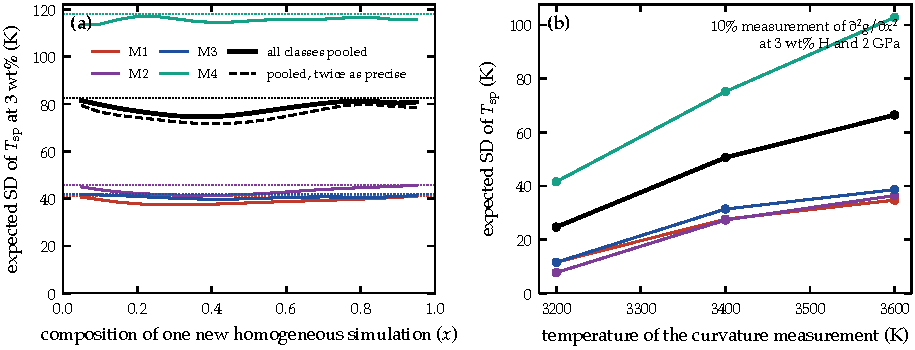
\includegraphics[width=\textwidth]{fig4_1_design}
\thesiscaption{Simulations that would constrain the spinodal.}{Expected posterior standard
deviation of the spinodal temperature of a 3\,wt\% parcel at 2\,GPa after (a) one new
homogeneous simulation of excess enthalpy, entropy and volume at composition $x$, for each
model class (thin lines) and all classes pooled (thick line; dotted lines: current values),
and (b) a measurement of the composition curvature $\partial^2 g/\partial x^2$ at the baseline
composition with 10\% precision, at three temperatures. Linear-Gaussian screen of the
recalibration samples.}
\label{fig:design}
\end{figure*}

A direct measurement of the curvature is more powerful. At 2\,GPa and \curvT{}\,K, a 10\%
measurement of $\partial^2 g/\partial x^2$ would reduce the standard deviation to
\curvSdPooled{}\,K. At this temperature \curvFracStable{}\% of the posterior samples leave the
baseline parcel locally stable: \curvFracMeta{}\% metastable and \curvFracOnePhase{}\% still one
phase. The curvature is accessible without a free-energy model, from the
long-wavelength limit of the Bhatia--Thornton concentration--concentration structure factor,
$S_{cc}(0) = RT/(\partial^2 g/\partial x^2)$ per mole of mixing units
\cite{bhatia1970,kirkwood1951}. Homogeneous DFT-MD simulations of the metastable parcel, in
cells large enough to sample composition fluctuations over several nanometres, could measure
it. Simulations below $T_C$ would also test the assumption of temperature-independent excess
enthalpy and entropy, which all four model classes share.

Even a measured spinodal fixes only the limit of the delay. Its actual length requires the
interfacial tension and the mobility of the mixture. The interface fluctuations in the
existing coexistence simulations could constrain the tension, because their magnitude is
related to it \cite{gilmore2026}. Together
they give nucleation rates through classical nucleation theory \cite{kashchiev2000}, which an
evolution model can then use in place of the two limiting cases studied here.

\chapter{Conclusion}\label{ch:conclusion}

The study of sub-Neptune exoplanets occupies a critical intersection between geophysics and
atmospheric science. This work has demonstrated that the release of hydrogen from a miscible
sub-Neptune interior cannot be timed from equilibrium miscibility data alone. Between the
equilibrium onset of exsolution and the loss of local stability lies a metastable window,
and its width is set by a part of the free energy that the existing simulations do not
sample. By utilizing the \Atm{} framework to compute binodals, spinodals and their
uncertainties for H$_2$--MgSiO$_3$ parcels across local hydrogen mass fractions of 0.1--20\%
and pressures of 2--10\,GPa, we have constrained the thermodynamic limits on hydrogen
exsolution during the cooling of the magma ocean. This chapter summarizes the primary
insights derived from this modeling and discusses their implications for interpreting
observations.

\section{Summary of Findings}

Our modeling yields four primary conclusions regarding the exsolution of hydrogen from
sub-Neptune interiors.

\subsection{A Composition-Consistent Mixing Model}

We implemented the final 2026 hydrogen--silicate mixing model in \Atm{}. The published model
uses oxide units, whereas \Atm{} uses MgSiO$_3$ formula units, and the conversion must act on
the extensive free energy, not only on the compositions. With this conversion our
implementation reproduces the published phase diagram with an RMS residual of \digRms{}\,K.
Without it,
the metastable interval of the baseline parcel is about nine times too short.

\subsection{The Metastable Window}

With the published fit, a parcel with 3\,wt\% local hydrogen at 2\,GPa enters the miscibility
gap at \pubTbTwo{}\,K and becomes unstable at \pubTspTwo{}\,K. Over this \pubIntTwo{}\,K
interval, delayed exsolution could withhold up to \pubFhTwo{}\% of its hydrogen from
separation. In the published fit, parcels with less than \pubThreshold{}\,wt\% hydrogen never
become unstable, so their separation always requires nucleation; in the refits this threshold
lies lower.

\subsection{The Source Data Do Not Fix the Window}

The published fit departs from its own source simulations in two places: the compositions of
the two runs closest to the critical curve, where the source table and figure also disagree,
and the excess volume, which is about half the value that the fitted pressure scale implies.
Refitting the same model form to all source data shortens the interval to
\IntMOneTable{}\,K (68\% range \IntMOneTableLo{}--\IntMOneTableHi{}\,K). Across four smooth
model classes and six data treatments, the median interval ranges from \IntRangeLo{} to
\IntRangeHi{}\,K, and the most flexible class still allows the published value. The window
depends on the asymmetry, the excess entropy and the strength of the interaction together, and
the coexisting compositions and the homogeneous simulations pull these in different
directions.

\subsection{The Spinodal Is Not Identifiable from Coexistence Data}

A free-energy perturbation that leaves every equilibrium observable unchanged still moves the
spinodal by tens to hundreds of kelvin. Any spinodal inferred from coexistence data is
therefore a property of the assumed functional form. The curvature inside the miscibility gap
has to be measured, not inferred.

\section{Implications for Observations}

These findings introduce a new uncertainty into the interpretation of young sub-Neptunes.
Evolution models with hydrogen--silicate miscibility time the release of hydrogen with the
equilibrium binodal. If nucleation is suppressed, the release can lag by up to several hundred
kelvin of cooling and then occur abruptly.

Therefore, observational constraints from instruments such as JWST should be interpreted
within a coupled framework:
\begin{enumerate}
\item \textbf{Radius evolution:} Inflation of the envelope by exsolved hydrogen may set in later
than equilibrium models predict. The demographic tests proposed for young sub-Neptunes
\cite{rogers2026} should therefore include the metastable window as a systematic
uncertainty.
\item \textbf{Atmospheric composition:} A delayed and abrupt supply of hydrogen would
temporarily lower the mean molecular weight and shift the carbon speciation toward CH$_4$, in
line with the hydrogen-budget dependence found in our thesis \cite{laga2025}. Such a signal
requires efficient transport from the interior and remains untested.
\item \textbf{Interpretive caution:} Because the window is not identifiable from present data,
atmospheric or radius signatures should not yet be interpreted as evidence for or against
spinodal decomposition.
\end{enumerate}

\section{Future Outlook}

While this work establishes a thermodynamic bound on delayed hydrogen exsolution,
the sub-Neptune environment remains complex. The current models assume a binary
H$_2$--MgSiO$_3$ mixture with temperature-independent excess enthalpy and entropy. Future
simulations should measure the curvature of the homogeneous free energy inside the miscibility
gap directly, through the concentration structure factor, and test the temperature dependence
of the excess properties below $T_C$. The interfacial tension and mobility then fix nucleation
rates, which an evolution model can use instead of the two limiting cases studied here.
Lastly, as the magma ocean solidifies, the exsolution of incompatible volatiles could lead to
late-stage atmospheric inflation. This, too, should be incorporated as a time-dependent
evolution of the cooling and crystallizing magma ocean, coupled to the atmospheric chemistry
of \Atm{}. Despite these open questions, this work highlights that accurately predicting when
a sub-Neptune releases its hydrogen requires a fundamental understanding of the metastable
states of its interior.


% ======================================================================= appendices
\onecolumn
\appendixmodetrue
\phantomsection\addcontentsline{toc}{chapter}{Appendices}
\thispagestyle{plain}
\vspace*{\fill}
\begin{center}{\bfseries\Huge Appendices}\end{center}
\vspace*{\fill}
\clearpage
\addtocontents{toc}{\protect\setcounter{tocdepth}{0}}
\appendix
\chapter{Thermodynamics of the Mixing Model}\label{app:thermo}

This appendix presents a self-contained theoretical framework for the hydrogen--silicate
mixing model used in \texttt{Atmodeller}. It unifies the free energy, the composition basis,
the chemical potentials and the stability conditions. The goal is to provide a physically
transparent explanation of why the binodal and the spinodal of the published model behave as
they do, and of which parts of that behaviour come from the model form rather than from the
data.

\section{Chemical Potentials on the Oxide Basis}

For a binary mixture of oxide units (component 1) and H$_2$ (component 2), with
$g_{\rm mix}(x)$ per mole of mixing units and $x$ the H$_2$ fraction, the chemical
potentials relative to the pure components are
\begin{equation}
\mu_1 = g_{\rm mix} - x\,g_{\rm mix}', \qquad \mu_2 = g_{\rm mix} + (1-x)\,g_{\rm mix}'.
\end{equation}
For Eq.~(\ref{eq:gs26}) with $f = 1-T/\tau+P/\pi$, the excess parts are
\begin{align}
\mu_1^{\rm ex} &= f\,x^2\left[B + 2(A-B)(1-x)\right],\\
\mu_2^{\rm ex} &= f\,(1-x)^2\left[A + 2(B-A)x\right],
\end{align}
which is equation~14 of \cite{gilmore2026} written for both components.

\section{Conversion to Native Formula Units}

\texttt{Atmodeller} counts $n_{\rm MgSiO_3}$ and $n_{\rm H_2}$. With
$G = (2n_{\rm MgSiO_3}+n_{\rm H_2})\,g_{\rm mix}(x)$ and
$x = n_{\rm H_2}/(2n_{\rm MgSiO_3}+n_{\rm H_2})$,
\begin{equation}
\frac{\partial G}{\partial n_{\rm MgSiO_3}} = 2\mu_1, \qquad
\frac{\partial G}{\partial n_{\rm H_2}} = \mu_2 .
\end{equation}
Per native mole, $h(y) = (2-y)\,g_{\rm mix}(x(y))$ with $x = y/(2-y)$ and
$dx/dy = 2/(2-y)^2$. Differentiating twice gives
\begin{equation}
h''(y) = \frac{4\,g_{\rm mix}''(x)}{(2-y)^3}.
\end{equation}
The curvature changes magnitude but not sign, so the spinodal is the same in both bases, as it
must be. The coexisting compositions are also the same once converted with
Eq.~(\ref{eq:basis}). Importing the published parameters without the factor $2-y$, as in our
incorrect-basis control, changes the free energy itself and therefore moves both curves.

\section{Spinodal Temperature and Its Threshold}

The excess curvature of Eq.~(\ref{eq:w}) is linear in composition,
\begin{equation}
W''(x) = 2B - 4A + 6(A-B)\,x .
\end{equation}
Setting $g_{\rm mix}'' = 0$ gives Eq.~(\ref{eq:tsp}). A positive spinodal temperature
requires $W''(x) < 0$, that is
\begin{equation}
x > x_{\rm min} = \frac{2B-4A}{6(B-A)} = 0.262
\end{equation}
for the published parameters. This corresponds to $w = \pubThreshold{}$\,wt\% local hydrogen.
Below this threshold a parcel can still separate in equilibrium, but its homogeneous state
never becomes unstable: separation there always requires nucleation.

\section{Why the Withheld Fraction Does Not Depend on Pressure}

Write $g_{\rm mix}/(RT) = s(x) + r\,W(x)$, with $s$ the ideal term and
\begin{equation}
r(T,P) = \frac{1 - T/\tau + P/\pi}{RT}.
\end{equation}
Phase equilibrium and stability depend on $T$ and $P$ only through $r$. At fixed composition
the spinodal fixes $r_{\rm sp} = -1/[x(1-x)W''(x)]$, and the binodal fixes another value
$r_b(x)$. Solving $r(T,P) = r_\ast$ gives
\begin{equation}
T_\ast(x,P) = \frac{1+P/\pi}{R\,r_\ast + 1/\tau} = T_\ast(x,0)\left(1+\frac{P}{\pi}\right).
\end{equation}
Both onset temperatures therefore scale with $1+P/\pi$, and the coexisting compositions at the
spinodal, hence $f_{\rm H}$, are the same at every pressure. The numerical invariance of
$f_{\rm H}$ (Section~\ref{sec:inventory}) is a consequence of this separable form, not
independent evidence. Classes M3 and M4 share it, because all their terms scale with the
same factor; class M2 does not.

\section{Critical Point}

At the critical point both the second and third derivatives of $g_{\rm mix}$ vanish. For
Eq.~(\ref{eq:gs26}) this gives equations~17--19 of \cite{gilmore2026}: the ratio $B/A$ fixes
the critical composition, here $x_C = \pubXc{}$ ($w = \pubWc{}$\,wt\%), and
\begin{equation}
T_C(P) = T_C^0\left(1+\frac{P}{\pi}\right), \qquad T_C^0 = \pubTcZero{}\,{\rm K}.
\end{equation}
The critical temperature is the same whichever component carries $A$; the critical
composition is not.

\section{Curvature Change of the Identifiability Perturbation}

For the perturbation of Eq.~(\ref{eq:bump}) with gap width $\Delta x = x_{\rm rich} -
x_{\rm poor}$,
\begin{equation}
\frac{\partial^2 \delta g}{\partial x^2}
= \lambda B_{\rm gap}\,\frac{384\,u(1-u)(1-5u+5u^2)}{\Delta x^2}.
\end{equation}
The change is negative in the middle of the gap ($0.28 < u < 0.72$) and positive near its
edges, so the perturbation can move the spinodal in either direction. This is why the 3\,wt\% spinodal
rises while the 5\,wt\% spinodal falls in Figure~\ref{fig:identifiability}. The value,
first and second derivatives of $\delta g$ vanish at $u=0$ and $u=1$, which keeps every
equilibrium quantity unchanged.

\chapter{Source Data and Audit Tables}\label{app:source}

This appendix reproduces the source simulations of Gilmore \& Stixrude \cite{gilmore2026} that
enter the audit and the recalibration, next to the predictions of the published fit. The
phase-coexistence runs contain 27 MgSiO$_3$ formula units and 92 to 219 hydrogen atoms; the
homogeneous runs contain 135 to 160 atoms. All
compositions are H$_2$ mole fractions $x$ on the oxide basis (Eq.~\ref{eq:x}).

\section{Phase-Coexistence Runs}

Table~\ref{tab:ed1} lists all 14 phase-coexistence runs. For runs that kept two phases it gives
the composition of the H-poor and H-rich phase from ED Table~1 and, where they differ, from the
digitized Figure~2a. For runs that became homogeneous it gives the bulk composition in
parentheses. The last column is the published critical temperature at the run pressure minus
the run temperature: positive values mean the model places the run below $T_C$.

\begin{table}[h]
\thesiscaption{Phase-coexistence runs of ED Table~1 and the published fit.}{Pressure
uncertainties in the last digits are given in parentheses. ``same'' means that the digitized
Figure~2a agrees with the table to within 0.001.}
\label{tab:ed1}
\small\centering
\begin{tabular}{@{}rrcllll@{}}
\toprule
$P$ (GPa) & $T$ (K) & Phases & ED Table~1 $x$ & Figure~2a $x$ & Published fit $x$ &
$T_C - T$ (K)\\
\midrule
\inputtable{tables/ed_table1.tex}
\bottomrule
\end{tabular}
\end{table}

In every two-phase run the per-phase atom numbers of ED Table~1 add up to the full simulation
cell, to within one atom. Each atom, including those in the two interfaces, is therefore
assigned to one of the two phases. For the 2.05 and 9.58\,GPa runs the table and the figure
agree to within \digMarker{}. For the 1.65 and 5.14\,GPa runs, which lie closest to the
critical curve, they differ by up to 0.07.

\section{Homogeneous Excess Properties}

Table~\ref{tab:homogeneous} lists the excess properties reconstructed from ED Table~2 per mole
of mixing units. The uncertainties include the shared endmember errors and the pressure-offset
systematic described in Section~\ref{sec:recalibration}. The enthalpy entries of different
compositions are correlated with coefficients of 0.48 to 0.76, the volumes with 0.48 to 0.78.

\begin{table}[h]
\thesiscaption{Excess properties of the homogeneous simulations at 5.06--5.08\,GPa and
4,000\,K}{(ED Table~2), with 1$\sigma$ uncertainties, next to the published fit.}
\label{tab:homogeneous}
\small\centering
\begin{tabular}{@{}lllllll@{}}
\toprule
& \multicolumn{2}{c}{$H_{\rm ex}$ (kJ\,mol$^{-1}$)} &
\multicolumn{2}{c}{$S_{\rm ex}$ (J\,mol$^{-1}$\,K$^{-1}$)} &
\multicolumn{2}{c}{$V_{\rm ex}$ (cm$^3$\,mol$^{-1}$)}\\
\cmidrule(lr){2-3}\cmidrule(lr){4-5}\cmidrule(lr){6-7}
$x$ & simulation & fit & simulation & fit & simulation & fit\\
\midrule
\inputtable{tables/homogeneous.tex}
\bottomrule
\end{tabular}
\end{table}

\chapter{Recalibration Details}\label{app:recalibration}

This appendix documents the priors, the sampler and the best-fitting parameters of the
recalibration of Section~\ref{sec:recalibration}.

\section{Priors}

All priors are uniform. For class M1, $A$ lies between $-300$ and 1,500\,kJ\,mol$^{-1}$ and $B$
between $-300$ and 3,000\,kJ\,mol$^{-1}$. For the other classes the leading coefficients lie
between $-300$ and 3,000\,kJ\,mol$^{-1}$, and higher Redlich--Kister terms within
$\pm2{,}000$\,kJ\,mol$^{-1}$. The
inverse temperature scale $1/\tau$ lies between 0 and $10^{-3}$\,K$^{-1}$ and the inverse
pressure scale $1/\pi$ between $-0.25$ and $0.1$\,GPa$^{-1}$. For class M2 the subregular
entropy coefficients lie between $-200$ and 800\,J\,mol$^{-1}$\,K$^{-1}$ and the volume
coefficients between $-60$ and 30\,cm$^3$\,mol$^{-1}$. Parameter sets for which the homogeneous
free energy develops more than one unstable composition interval at any evaluated state are
outside every model class and receive zero probability.

\section{Sampler and Convergence}

Each fit starts from the best of eight Nelder--Mead optimizations around the published
parameters. Eight adaptive Metropolis chains \cite{haario2001} then run 12,000 steps each.
During the first 3,000 steps the proposal covariance and scale adapt; these steps are
discarded. Every 30th later step is kept, which gives 2,400 posterior samples per fit. The
acceptance rate is about 0.2 in every fit. The largest split-chain $\hat R$ over all
parameters and derived quantities of all fits is \maxRhat{}.

\section{Best-Fitting Parameters}

Table~\ref{tab:map} lists the best-fitting (MAP) parameters of class M1 for each data
treatment, next to the published values.

\begin{table}[h]
\thesiscaption{Best-fitting parameters of the published model form (class M1).}{$B/A$ sets
the asymmetry and the critical composition; $\tau$ and $\pi$ set the temperature and pressure
scales.}
\label{tab:map}
\small\centering
\begin{tabular}{@{}lrrrrr@{}}
\toprule
Fit & $A$ (kJ\,mol$^{-1}$) & $B$ (kJ\,mol$^{-1}$) & $B/A$ & $\tau$ (K) & $\pi$ (GPa)\\
\midrule
\inputtable{tables/map_parameters.tex}
\bottomrule
\end{tabular}
\end{table}

\chapter{Reproducibility}\label{app:repro}

This appendix lists how every number and figure in this draft is produced. All paths are
relative to the repository root. The analysis used Python~3.13 with the package versions
recorded in \texttt{research/spinodal\_onset/outputs/provenance.json}.

\section{Pipeline}

\begin{enumerate}
\item \texttt{run\_study.py} computes the onset grid, the cooling paths, the source-data audit,
the homogeneous audit, the stress cases and the native \texttt{Atmodeller} solves.
\item \texttt{identifiability.py} builds the perturbation of Eq.~(\ref{eq:bump}) and checks that
it leaves every equilibrium quantity unchanged.
\item \texttt{digitize\_source\_figure.py} digitizes Figure~2a of \cite{gilmore2026} and compares
it with our implementation.
\item \texttt{calibration.py} runs the recalibration (Section~\ref{sec:recalibration}); about
40 minutes of computation with eight worker processes.
\item \texttt{design.py} computes the design screen of Section~\ref{sec:design}.
\item \texttt{make\_paper\_figures.py} writes all figures, and \texttt{paper/make\_numbers.py}
writes the computed numbers and table bodies to \texttt{paper/numbers.tex} and
\texttt{paper/tables}.
\end{enumerate}

Most computed numbers in the text are macros generated from the output files, so rebuilding
the draft after a rerun updates the text with the figures. A few values are typed directly,
such as the bulk compositions of source runs and rounded ratios; they are listed with their
origin in Appendix~\ref{app:source} or follow from the macros.

\section{Commands}

\begin{verbatim}
uv sync --locked --all-extras --dev
PYTHONPATH=. uv run python research/spinodal_onset/run_study.py
PYTHONPATH=. uv run python research/spinodal_onset/identifiability.py
PYTHONPATH=. uv run python research/spinodal_onset/digitize_source_figure.py
PYTHONPATH=. uv run python research/spinodal_onset/calibration.py
PYTHONPATH=. uv run python research/spinodal_onset/design.py
PYTHONPATH=. uv run python research/spinodal_onset/make_paper_figures.py
PYTHONPATH=. uv run python research/spinodal_onset/paper/make_numbers.py
cd research/spinodal_onset/paper && tectonic -X compile main.tex
\end{verbatim}

\section{Data Provenance}

The ED Tables and Figure~2 of \cite{gilmore2026} are stored unmodified in
\texttt{research/spinodal\_onset/sources} with their SHA-256 hashes, source URLs and the
CC-BY-4.0 attribution. No source value was changed. Where the table and the figure disagree,
both are kept and analysed as separate data versions. The thesis layout reuses the KU Leuven
title-page logo of the bachelor thesis. Its use should be checked against the current KU Leuven
style rules before the draft is submitted or shared beyond this repository.


% ======================================================================= references
\twocolumn
\appendixmodefalse
\phantomsection\addcontentsline{toc}{chapter}{References}
\markboth{References}{References}
{\small\bibliographystyle{plain}\bibliography{references}}

\end{document}
